% !TEX root = presentation.tex
\documentclass[aspectratio=169, 10pt]{beamer}

% ==============================================================================
% PACKAGES & SYSTEM SETUP
% ==============================================================================
\usepackage[utf8]{inputenc}
\usepackage[T1]{fontenc}
\usepackage{amsmath,amssymb}
\usepackage{graphicx}
\usepackage{booktabs}
\usepackage{tabularx}
\usepackage{colortbl}
\usepackage{tikz}
\usetikzlibrary{shapes.geometric,arrows.meta,positioning,calc,fit,backgrounds}
\usepackage[most]{tcolorbox}

% ==============================================================================
% COLOR PALETTE (EXACT PPTX / CANVA MATCHING)
% ==============================================================================
\definecolor{bgDark}{HTML}{071923}        % Deep Midnight Blue/Cyan Canvas
\definecolor{bgCard}{HTML}{0D2536}        % Dark Card Background
\definecolor{bgCardLight}{HTML}{14364F}   % Elevated Card / Border
\definecolor{cyanAccent}{HTML}{30AFFF}    % Electric Cyan Primary
\definecolor{cyanGlow}{HTML}{92EEFF}      % Ice Cyan Glow
\definecolor{textWhite}{HTML}{F5FBFF}     % Crisp High-Contrast White Text
\definecolor{textMuted}{HTML}{94A3B8}     % Secondary Muted Text
\definecolor{mintGreen}{HTML}{10B981}     % Success / High Accuracy Accent
\definecolor{amberWarn}{HTML}{F59E0B}     % Warning / Trade-off Accent
\definecolor{roseRed}{HTML}{EF4444}       % Error / Ground Truth Accent

% ==============================================================================
% BEAMER THEME & TYPOGRAPHY
% ==============================================================================
\setbeamercolor{background canvas}{bg=bgDark}
\setbeamercolor{normal text}{fg=textWhite}
\setbeamercolor{structure}{fg=cyanAccent}
\setbeamercolor{frametitle}{fg=textWhite, bg=bgDark}
\setbeamercolor{item}{fg=cyanAccent}
\setbeamercolor{subitem}{fg=cyanGlow}

\setbeamertemplate{navigation symbols}{}

% Custom slide header
\setbeamertemplate{frametitle}{
  \vspace{0.35cm}
  \begin{beamercolorbox}[wd=\paperwidth,leftskip=0.8cm,rightskip=0.8cm]{frametitle}
    {\fontsize{7.5pt}{9pt}\selectfont\color{cyanAccent}\textbf{\insertsectionhead}} \vskip1pt
    {\fontsize{15pt}{17pt}\selectfont\color{textWhite}\textbf{\insertframetitle}}
  \end{beamercolorbox}
}

% Custom slide footer
\setbeamertemplate{footline}{
  \leavevmode%
  \hbox{%
    \begin{beamercolorbox}[wd=0.72\paperwidth,ht=3ex,dp=1.5ex,leftskip=0.8cm]{normal text}%
      \fontsize{7pt}{8pt}\selectfont\color{textMuted}\textbf{DSP MIDTERM 2026} \;\textcolor{cyanAccent}{$\vert$}\; GROUP 08 \;\textcolor{cyanAccent}{$\vert$}\; VOICE ACTIVITY DETECTION
    \end{beamercolorbox}%
    \begin{beamercolorbox}[wd=0.28\paperwidth,ht=3ex,dp=1.5ex,rightskip=0.8cm]{normal text}%
      \hfill\fontsize{7.5pt}{8.5pt}\selectfont\color{cyanGlow}\textbf{\insertframenumber} \textcolor{textMuted}{/ \inserttotalframenumber}
    \end{beamercolorbox}%
  }%
  \vskip4pt%
}

% Custom itemize bullet
\setbeamertemplate{itemize item}{\textcolor{cyanAccent}{\textbf{\textbullet}}}
\setbeamertemplate{itemize subitem}{\textcolor{cyanGlow}{\textbf{--}}}

% ==============================================================================
% TCOLORBOX CARD STYLES
% ==============================================================================
\tcbset{
  darkcard/.style={
    enhanced,
    colback=bgCard,
    colframe=bgCardLight,
    arc=2.5mm,
    boxrule=0.8pt,
    left=6pt, right=6pt, top=6pt, bottom=6pt,
    coltext=textWhite
  },
  glowcard/.style={
    enhanced,
    colback=bgCard,
    colframe=cyanAccent,
    arc=2.5mm,
    boxrule=1.1pt,
    left=6pt, right=6pt, top=6pt, bottom=6pt,
    coltext=textWhite
  },
  mintcard/.style={
    enhanced,
    colback=bgCard,
    colframe=mintGreen,
    arc=2.5mm,
    boxrule=1.1pt,
    left=6pt, right=6pt, top=6pt, bottom=6pt,
    coltext=textWhite
  },
  warncard/.style={
    enhanced,
    colback=bgCard,
    colframe=amberWarn,
    arc=2.5mm,
    boxrule=1.1pt,
    left=6pt, right=6pt, top=6pt, bottom=6pt,
    coltext=textWhite
  },
  whiteframe/.style={
    enhanced,
    colback=white,
    colframe=cyanAccent,
    arc=2mm,
    boxrule=1.2pt,
    left=1pt, right=1pt, top=1pt, bottom=1pt
  },
  portraitframe/.style={
    enhanced,
    colback=bgDark,
    colframe=cyanAccent,
    arc=2.5mm,
    boxrule=1.1pt,
    left=0pt, right=0pt, top=0pt, bottom=0pt
  }
}

% ==============================================================================
% DOCUMENT METADATA
% ==============================================================================
\title{VOICE ACTIVITY DETECTION (VAD)}
\subtitle{Three Algorithms · One Unified Evaluation Benchmark}
\author{Group 03}
\institute{Digital Signal Processing Midterm Project 2026}
\date{October 2026}

\begin{document}

% ==============================================================================
% SLIDE 01: TITLE / COVER
% ==============================================================================
\section{DSP MIDTERM PROJECT REPORT · 2026}
\begin{frame}[plain]
  \vspace{0.4cm}
  \begin{center}
    {\fontsize{9pt}{11pt}\selectfont\color{cyanAccent}\textbf{DSP MIDTERM PROJECT REPORT $\cdot$ 2026}}\\[4pt]
    {\fontsize{22pt}{24pt}\selectfont\color{textWhite}\textbf{VOICE ACTIVITY DETECTION (VAD)}}\\[3pt]
    {\fontsize{11pt}{13pt}\selectfont\color{cyanGlow}\textbf{Three Algorithms $\cdot$ One Unified Evaluation Benchmark}}\\[14pt]
    
    \begin{columns}[T]
      \begin{column}{0.31\textwidth}
        \begin{tcolorbox}[glowcard]
          \centering
          {\fontsize{10pt}{12pt}\selectfont\color{cyanGlow}\textbf{Luong Duy Toan}}\\[3pt]
          {\fontsize{8.5pt}{10pt}\selectfont\color{textWhite}\textbf{Algorithm 01}}\\[2pt]
          {\fontsize{8pt}{9pt}\selectfont\color{textMuted}Hodgkinson $\cdot$ Binary Search}
        \end{tcolorbox}
      \end{column}
      
      \begin{column}{0.31\textwidth}
        \begin{tcolorbox}[glowcard]
          \centering
          {\fontsize{10pt}{12pt}\selectfont\color{cyanGlow}\textbf{Nguyen Anh Hoang}}\\[3pt]
          {\fontsize{8.5pt}{10pt}\selectfont\color{textWhite}\textbf{Algorithm 02}}\\[2pt]
          {\fontsize{8pt}{9pt}\selectfont\color{textMuted}Giannakopoulos $\cdot$ Histogram}
        \end{tcolorbox}
      \end{column}
      
      \begin{column}{0.31\textwidth}
        \begin{tcolorbox}[glowcard]
          \centering
          {\fontsize{10pt}{12pt}\selectfont\color{cyanGlow}\textbf{Truong Bui Dien}}\\[3pt]
          {\fontsize{8.5pt}{10pt}\selectfont\color{textWhite}\textbf{Algorithm 03}}\\[2pt]
          {\fontsize{8pt}{9pt}\selectfont\color{textMuted}Gaussian Bayes Separation}
        \end{tcolorbox}
      \end{column}
    \end{columns}
    
    \vspace{12pt}
    {\fontsize{8.5pt}{10pt}\selectfont\color{textMuted}\textbf{GROUP 08} $\;\vert\;$ 16 kHz Standard Audio $\;\vert\;$ Fully Pre-Executed Notebooks}
  \end{center}
\end{frame}

% ==============================================================================
% SLIDE 02: SHARED ARCHITECTURE
% ==============================================================================
\section{SHARED ARCHITECTURE $\cdot$ GROUP 03}
\begin{frame}
  \frametitle{Unified End-to-End DSP Pipeline}
  \begin{center}
    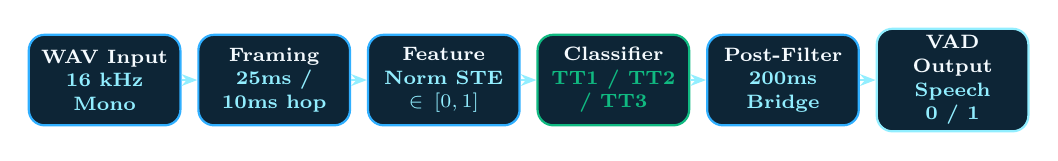
\begin{tikzpicture}[
      node distance=0.20cm,
      stage/.style={
        rectangle, rounded corners=2mm, fill=bgCard, draw=cyanAccent, line width=0.8pt,
        text=textWhite, align=center, font=\fontsize{7.5pt}{8.5pt}\selectfont\bfseries,
        minimum height=1.15cm, text width=1.75cm, inner sep=2.5pt
      },
      arrow/.style={-{Stealth[scale=0.75]}, draw=cyanGlow, line width=1pt}
    ]
      \node[stage] (s1) {WAV Input\\{\color{cyanGlow}\scriptsize 16 kHz Mono}};
      \node[stage, right=of s1] (s2) {Framing\\{\color{cyanGlow}\scriptsize 25ms / 10ms hop}};
      \node[stage, right=of s2] (s3) {Feature\\{\color{cyanGlow}\scriptsize Norm STE $\in [0, 1]$}};
      \node[stage, right=of s3, draw=mintGreen] (s4) {Classifier\\{\color{mintGreen}\scriptsize TT1 / TT2 / TT3}};
      \node[stage, right=of s4] (s5) {Post-Filter\\{\color{cyanGlow}\scriptsize 200ms Bridge}};
      \node[stage, right=of s5, draw=cyanGlow] (s6) {VAD Output\\{\color{cyanGlow}\scriptsize Speech 0 / 1}};

      \draw[arrow] (s1) -- (s2);
      \draw[arrow] (s2) -- (s3);
      \draw[arrow] (s3) -- (s4);
      \draw[arrow] (s4) -- (s5);
      \draw[arrow] (s5) -- (s6);
    \end{tikzpicture}
  \end{center}

  \vspace{6pt}
  \begin{columns}[T]
    \begin{column}{0.48\textwidth}
      \begin{tcolorbox}[darkcard, height=3.05cm, valign=top]
        {\fontsize{9pt}{10pt}\selectfont\color{cyanGlow}\textbf{Framing \& Feature Standard}}\\[4pt]
        {\fontsize{8pt}{10.5pt}\selectfont
        $\bullet$ Sampling: $16\text{ kHz}$ mono audio standard\\[3pt]
        $\bullet$ Frame size: 25 ms (400 samples)\\[3pt]
        $\bullet$ Frame hop: 10 ms (160 samples, 60\% overlap)\\[3pt]
        $\bullet$ Feature: Normalized STE $\in [0, 1]$}
      \end{tcolorbox}
    \end{column}

    \begin{column}{0.48\textwidth}
      \begin{tcolorbox}[darkcard, height=3.05cm, valign=top]
        {\fontsize{9pt}{10pt}\selectfont\color{cyanGlow}\textbf{Decision \& Post-Processing}}\\[4pt]
        {\fontsize{8pt}{10.5pt}\selectfont
        $\bullet$ Silence rule: Minimum duration $\ge 200\text{ ms}$\\[3pt]
        $\bullet$ Speech floor: Duration threshold $\ge 50\text{ ms}$\\[3pt]
        $\bullet$ Bridge rule: Connects short speech pauses\\[3pt]
        $\bullet$ Evaluation: MAE \& RMSE against .lab}
      \end{tcolorbox}
    \end{column}
  \end{columns}
\end{frame}

% ==============================================================================
% SLIDE 03: STUDENT 1 COVER
% ==============================================================================
\section{STUDENT 1 $\cdot$ ALGORITHM 01}
\begin{frame}
  \frametitle{Fixed Global Energy Threshold}
  \begin{columns}[c]
    \begin{column}{0.62\textwidth}
      \begin{tcolorbox}[glowcard]
        {\fontsize{13pt}{15pt}\selectfont\color{cyanGlow}\textbf{Luong Duy Toan}}\\[3pt]
        {\fontsize{9.5pt}{11pt}\selectfont\color{textWhite}\textbf{Algorithm 01 $\cdot$ Hodgkinson (2012)}}\\[6pt]
        {\fontsize{8.5pt}{10pt}\selectfont\color{textMuted}
        $\bullet$ Reference: CS425 Audio \& Speech Processing\\[3pt]
        $\bullet$ Approach: Global Short-Time Energy threshold\\[3pt]
        $\bullet$ Optimization: Iterative Binary Search on training set\\[3pt]
        $\bullet$ Objective: Minimize boundary MAE across 4 train signals\\[3pt]
        $\bullet$ Outcome: Fast $O(1)$ runtime decision per frame}
      \end{tcolorbox}
    \end{column}

    \begin{column}{0.34\textwidth}
      \begin{center}
        \begin{tcolorbox}[portraitframe]
          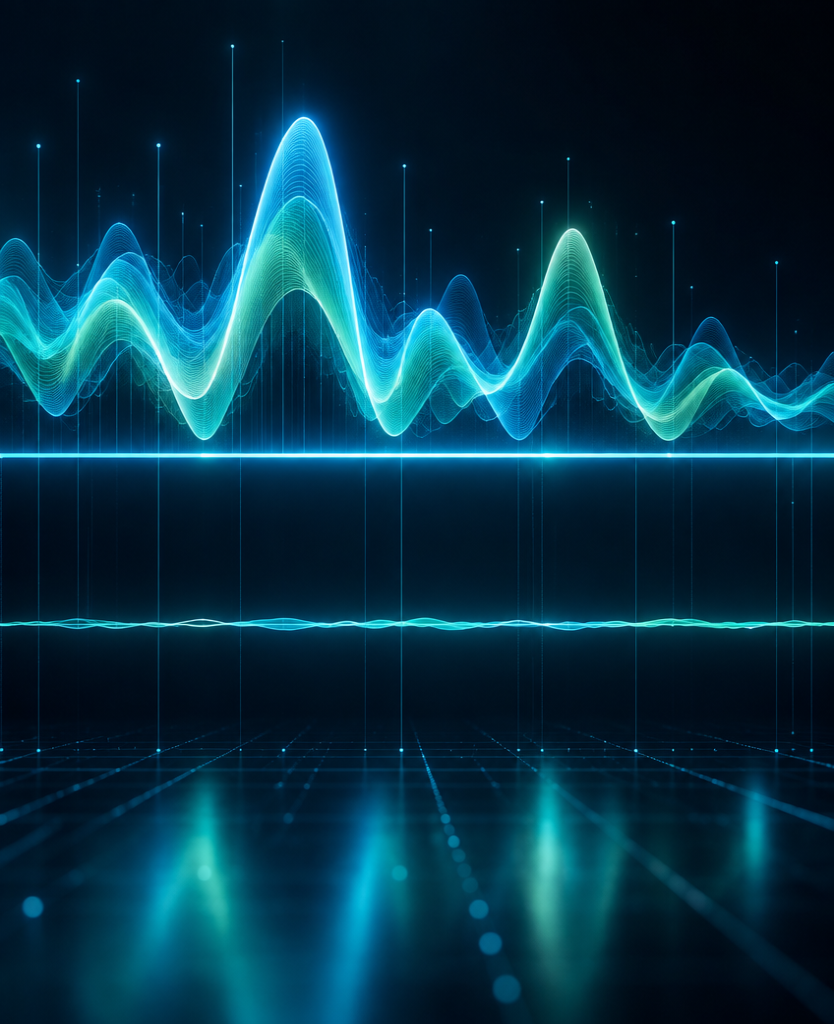
\includegraphics[width=\textwidth, height=4.2cm, keepaspectratio]{figures/student1_portrait.png}
        \end{tcolorbox}
      \end{center}
    \end{column}
  \end{columns}
\end{frame}

% ==============================================================================
% SLIDE 04: ALG 1 CORE METHOD
% ==============================================================================
\section{ALG 1 $\cdot$ CORE METHOD}
\begin{frame}
  \frametitle{Binary Search Optimization for $T_{\text{opt}}$}
  \begin{center}
    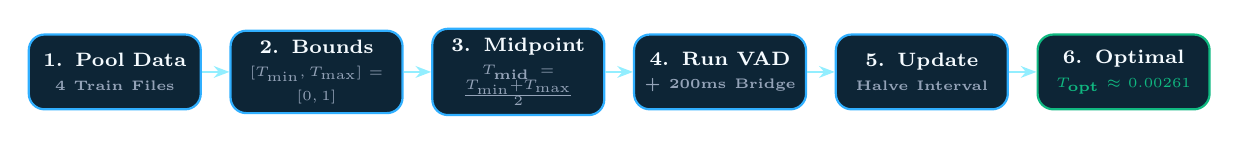
\begin{tikzpicture}[
      node distance=0.35cm,
      stepnode/.style={
        rectangle, rounded corners=2mm, fill=bgCard, draw=cyanAccent, line width=0.8pt,
        text=textWhite, align=center, font=\fontsize{7.5pt}{8.5pt}\selectfont\bfseries,
        minimum height=0.95cm, text width=1.95cm
      },
      flowarr/.style={-{Stealth[scale=0.75]}, draw=cyanGlow, line width=1pt}
    ]
      \node[stepnode] (p1) {1. Pool Data\\{\color{textMuted}\tiny 4 Train Files}};
      \node[stepnode, right=of p1] (p2) {2. Bounds\\{\color{textMuted}\tiny $[T_{\min}, T_{\max}]=[0, 1]$}};
      \node[stepnode, right=of p2] (p3) {3. Midpoint\\{\color{textMuted}\tiny $T_{\text{mid}}=\frac{T_{\min}+T_{\max}}{2}$}};
      \node[stepnode, right=of p3] (p4) {4. Run VAD\\{\color{textMuted}\tiny + 200ms Bridge}};
      \node[stepnode, right=of p4] (p5) {5. Update\\{\color{textMuted}\tiny Halve Interval}};
      \node[stepnode, right=of p5, draw=mintGreen] (p6) {6. Optimal\\{\color{mintGreen}\tiny $T_{\text{opt}} \approx 0.00261$}};

      \draw[flowarr] (p1) -- (p2);
      \draw[flowarr] (p2) -- (p3);
      \draw[flowarr] (p3) -- (p4);
      \draw[flowarr] (p4) -- (p5);
      \draw[flowarr] (p5) -- (p6);
    \end{tikzpicture}
  \end{center}

  \vspace{8pt}
  \begin{columns}[T]
    \begin{column}{0.48\textwidth}
      \begin{tcolorbox}[darkcard]
        {\fontsize{9pt}{10pt}\selectfont\color{cyanGlow}\textbf{Optimization Formulation}}\\[3pt]
        {\fontsize{8.5pt}{10pt}\selectfont
        $\bullet$ Cost function: $J(T) = \frac{1}{4}\sum_{k=1}^4 \text{MAE}_k(T)$\\[2pt]
        $\bullet$ Direction: Signed total speech duration error\\[2pt]
        $\bullet$ Convergence: Stops at 40 iterations ($\Delta T < 10^{-6}$)}
      \end{tcolorbox}
    \end{column}

    \begin{column}{0.48\textwidth}
      \begin{tcolorbox}[mintcard]
        {\fontsize{9pt}{10pt}\selectfont\color{mintGreen}\textbf{Learned Threshold Result}}\\[3pt]
        {\fontsize{8.5pt}{10pt}\selectfont
        $\bullet$ Global threshold: $\mathbf{T_{\text{opt}} = 0.00261}$\\[2pt]
        $\bullet$ Monotonic loss reduction on training audio\\[2pt]
        $\bullet$ Fixed threshold applied across all test recordings}
      \end{tcolorbox}
    \end{column}
  \end{columns}
\end{frame}

% ==============================================================================
% SLIDE 05: ALG 1 EXPERIMENTS
% ==============================================================================
\section{ALG 1 $\cdot$ EXPERIMENTS}
\begin{frame}
  \frametitle{Accuracy on Matched Noise Levels (4 Test Files)}
  \begin{columns}[c]
    \begin{column}{0.64\textwidth}
      \begin{tcolorbox}[whiteframe]
        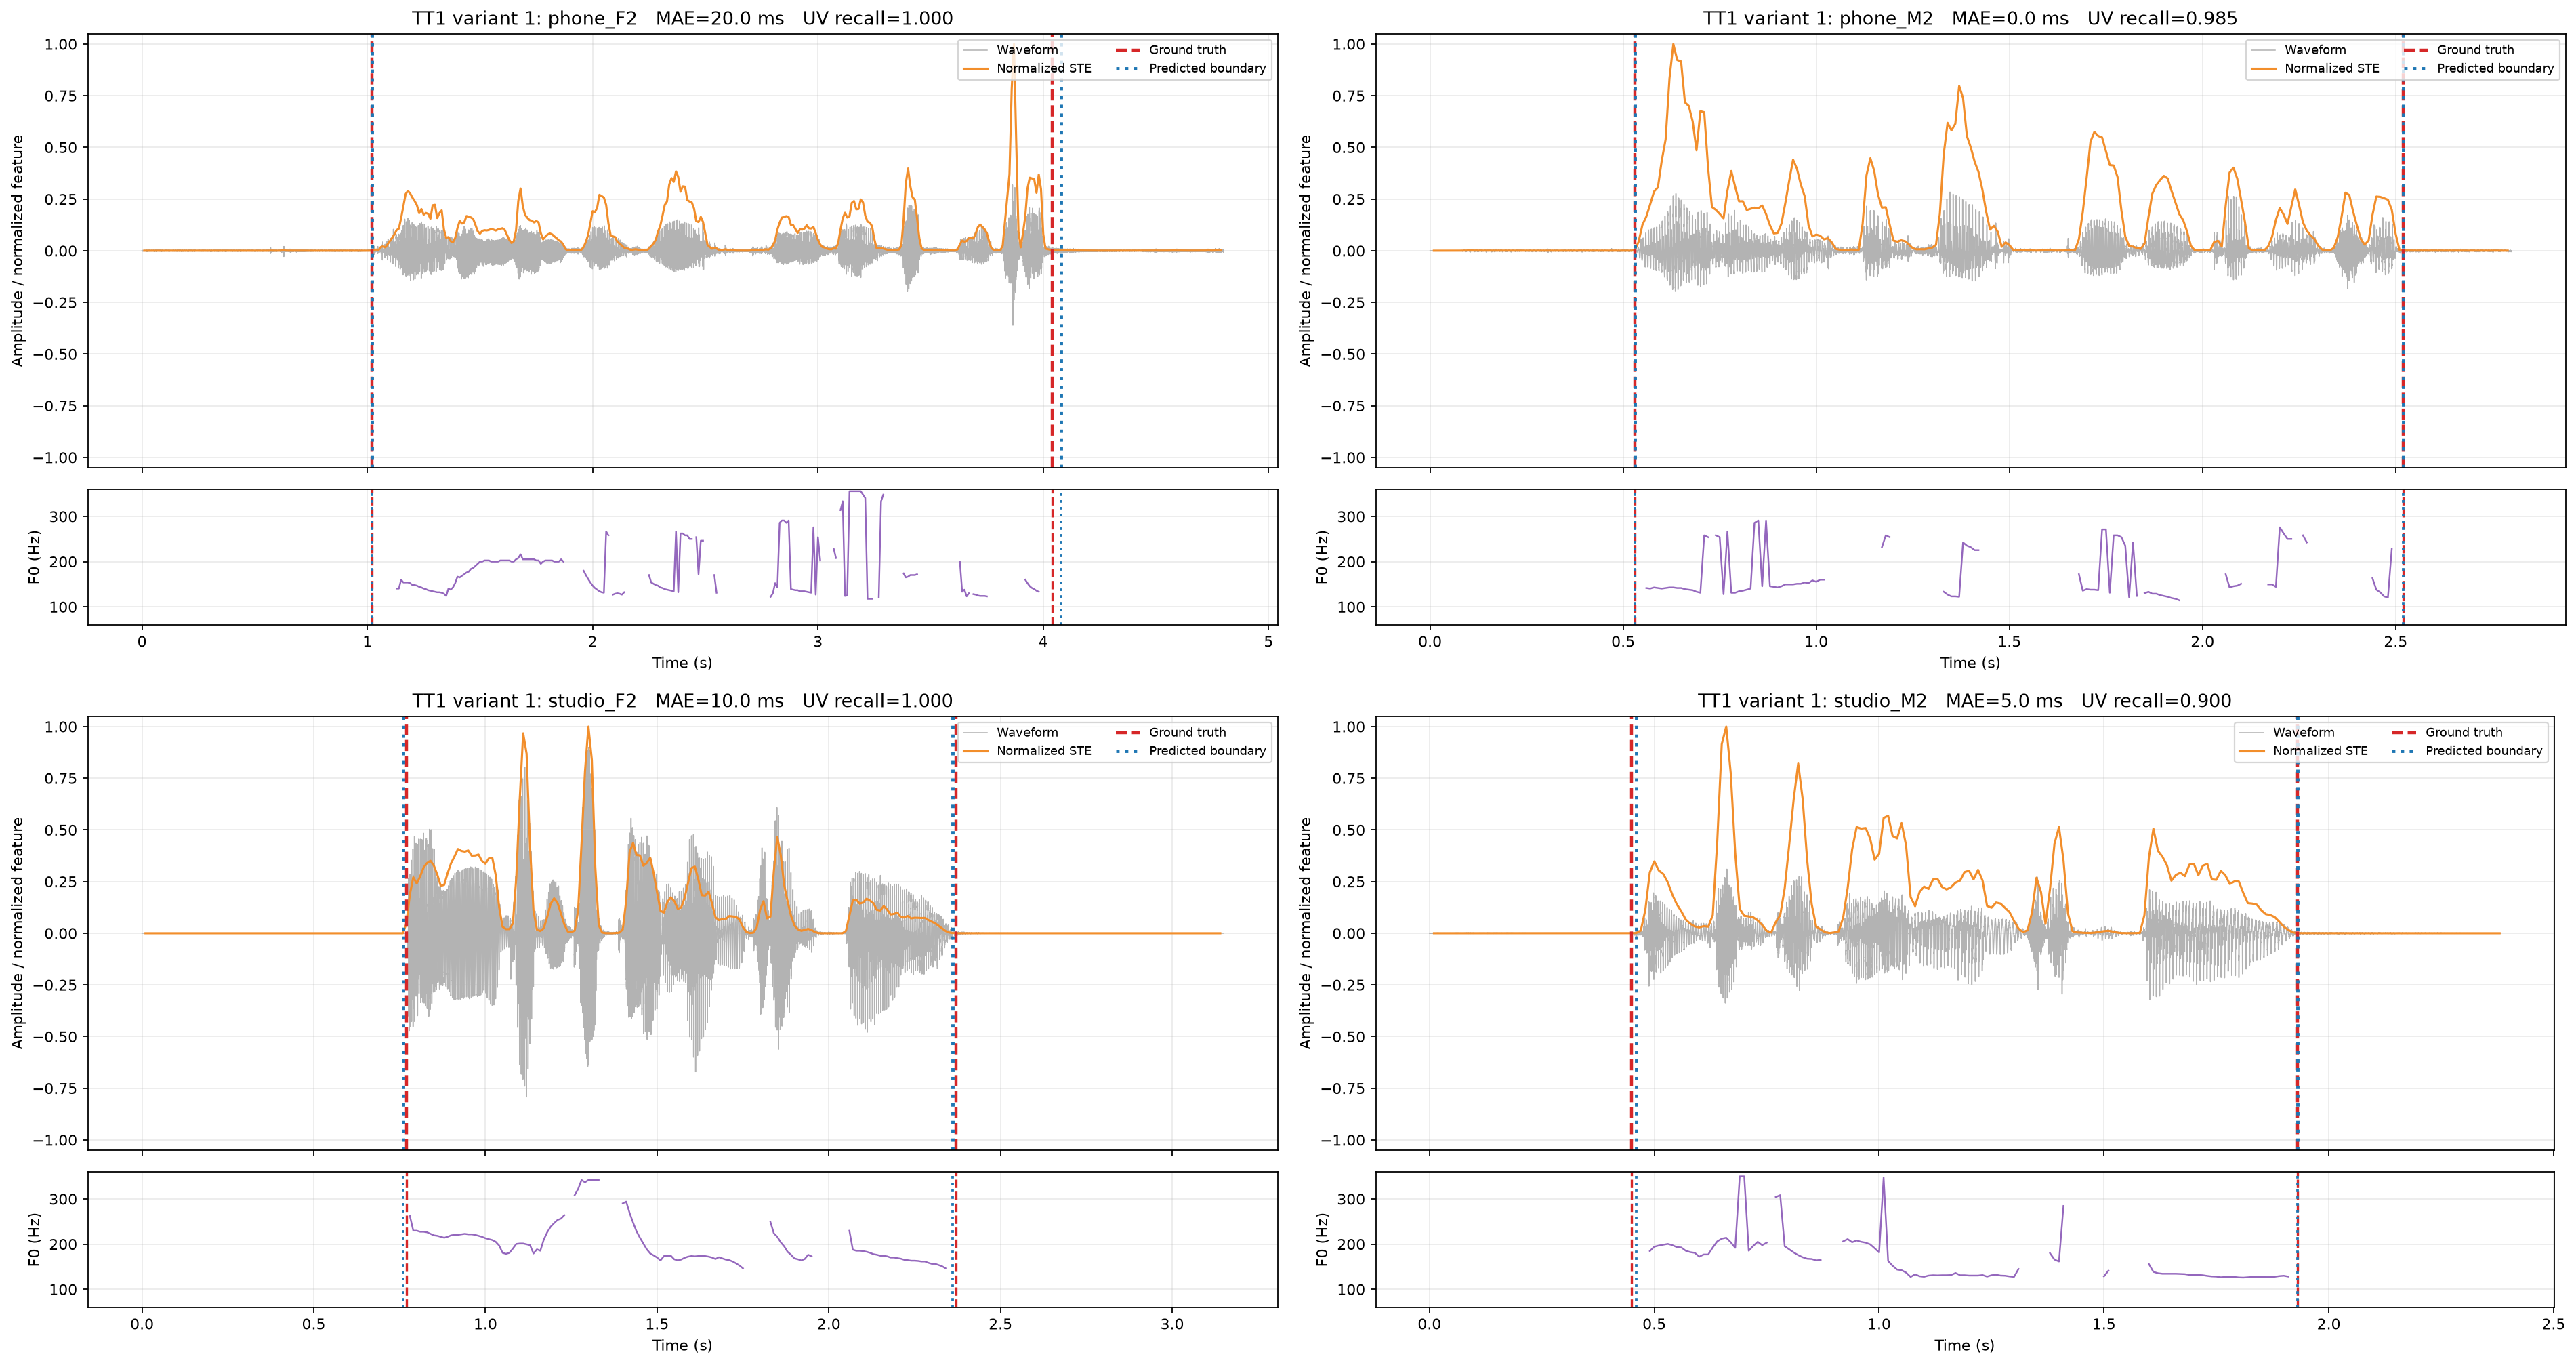
\includegraphics[width=\textwidth, height=4.6cm, keepaspectratio]{figures/tt1_composite.png}
      \end{tcolorbox}
    \end{column}

    \begin{column}{0.34\textwidth}
      \begin{tcolorbox}[mintcard]
        {\fontsize{9pt}{10pt}\selectfont\color{mintGreen}\textbf{Accurate Performance}}\\[2pt]
        {\fontsize{8pt}{9.5pt}\selectfont
        $\bullet$ Mean MAE: \textbf{8.75 ms} (6.25 ms ext)\\[2pt]
        $\bullet$ Sharp boundaries on studio files\\[2pt]
        $\bullet$ phone\_M2 MAE = \textbf{0.0 ms} (exact grid)}
      \end{tcolorbox}
      \vskip4pt
      \begin{tcolorbox}[warncard]
        {\fontsize{9pt}{10pt}\selectfont\color{amberWarn}\textbf{Limitation}}\\[2pt]
        {\fontsize{8pt}{9.5pt}\selectfont
        $\bullet$ Fixed threshold sensitive to SNR\\[2pt]
        $\bullet$ Trailing breath lag in phone\_F2}
      \end{tcolorbox}
    \end{column}
  \end{columns}
\end{frame}

% ==============================================================================
% SLIDE 06: ALG 1 CRITIQUE
% ==============================================================================
\section{ALG 1 $\cdot$ CRITIQUE}
\begin{frame}
  \frametitle{Strengths, Weaknesses, and Best Use Case}
  \begin{columns}[T]
    \begin{column}{0.31\textwidth}
      \begin{tcolorbox}[mintcard]
        \centering
        {\fontsize{9.5pt}{11pt}\selectfont\color{mintGreen}\textbf{STRENGTHS}}\\[4pt]
        \raggedright{\fontsize{8.5pt}{10pt}\selectfont
        $\bullet$ Ultra-fast $O(1)$ frame check\\[3pt]
        $\bullet$ Zero runtime memory overhead\\[3pt]
        $\bullet$ Highest boundary accuracy}
      \end{tcolorbox}
    \end{column}

    \begin{column}{0.31\textwidth}
      \begin{tcolorbox}[warncard]
        \centering
        {\fontsize{9.5pt}{11pt}\selectfont\color{amberWarn}\textbf{WEAKNESSES}}\\[4pt]
        \raggedright{\fontsize{8.5pt}{10pt}\selectfont
        $\bullet$ Rigid static threshold\\[3pt]
        $\bullet$ Zero adaptation to noise\\[3pt]
        $\bullet$ Degrades under severe SNR drop}
      \end{tcolorbox}
    \end{column}

    \begin{column}{0.31\textwidth}
      \begin{tcolorbox}[glowcard]
        \centering
        {\fontsize{9.5pt}{11pt}\selectfont\color{cyanGlow}\textbf{BEST USE CASE}}\\[4pt]
        \raggedright{\fontsize{8.5pt}{10pt}\selectfont
        $\bullet$ Low-power embedded MCUs\\[3pt]
        $\bullet$ Stationary studio environments\\[3pt]
        $\bullet$ Real-time streaming VAD}
      \end{tcolorbox}
    \end{column}
  \end{columns}
  
  \vspace{10pt}
  \begin{center}
    {\fontsize{8.5pt}{10pt}\selectfont\color{textMuted}\textbf{Key Lesson:} Simplicity is an asset when background noise is stationary.}
  \end{center}
\end{frame}

% ==============================================================================
% SLIDE 07: STUDENT 2 COVER
% ==============================================================================
\section{STUDENT 2 $\cdot$ ALGORITHM 02}
\begin{frame}
  \frametitle{Adaptive Energy Histogram}
  \begin{columns}[c]
    \begin{column}{0.62\textwidth}
      \begin{tcolorbox}[glowcard]
        {\fontsize{13pt}{15pt}\selectfont\color{cyanGlow}\textbf{Nguyen Anh Hoang}}\\[3pt]
        {\fontsize{9.5pt}{11pt}\selectfont\color{textWhite}\textbf{Algorithm 02 $\cdot$ Giannakopoulos (2014)}}\\[6pt]
        {\fontsize{8.5pt}{10pt}\selectfont\color{textMuted}
        $\bullet$ Reference: Silence Removal and Speech Segmentation\\[3pt]
        $\bullet$ Approach: Unsupervised STE energy histogram\\[3pt]
        $\bullet$ Mechanism: Dynamic threshold per recording via peaks\\[3pt]
        $\bullet$ Advantage: Zero ground-truth training required\\[3pt]
        $\bullet$ Tuning: Weighted valley parameter $W$ controls bias}
      \end{tcolorbox}
    \end{column}

    \begin{column}{0.34\textwidth}
      \begin{center}
        \begin{tcolorbox}[portraitframe]
          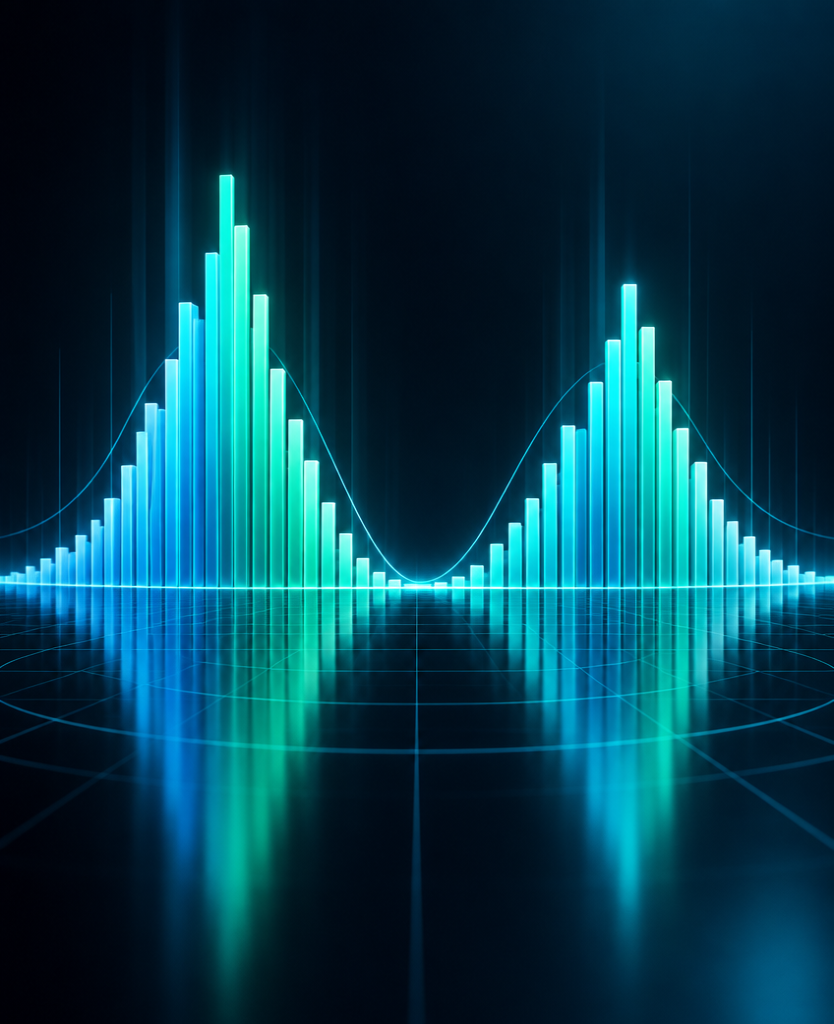
\includegraphics[width=\textwidth, height=4.2cm, keepaspectratio]{figures/student2_portrait.png}
        \end{tcolorbox}
      \end{center}
    \end{column}
  \end{columns}
\end{frame}

% ==============================================================================
% SLIDE 08: ALG 2 CORE METHOD
% ==============================================================================
\section{ALG 2 $\cdot$ CORE METHOD}
\begin{frame}
  \frametitle{Unsupervised Dual-Peak Energy Histogram}
  \begin{center}
    
\begin{tikzpicture}[
      node distance=0.35cm,
      stepnode/.style={
        rectangle, rounded corners=2mm, fill=bgCard, draw=cyanAccent, line width=0.8pt,
        text=textWhite, align=center, font=\fontsize{7.5pt}{8.5pt}\selectfont\bfseries,
        minimum height=0.95cm, text width=1.95cm
      },
      flowarr/.style={-{Stealth[scale=0.75]}, draw=cyanGlow, line width=1pt}
    ]
      \node[stepnode] (h1) {1. STE Norm\\{\color{textMuted}\tiny Per Audio File}};
      \node[stepnode, right=of h1] (h2) {2. Histogram\\{\color{textMuted}\tiny 100 Linear Bins}};
      \node[stepnode, right=of h2] (h3) {3. MA Filter\\{\color{textMuted}\tiny 5-Bin Smoothing}};
      \node[stepnode, right=of h3] (h4) {4. Find Peaks\\{\color{textMuted}\tiny $M_1$ (Sil), $M_2$ (Sp)}};
      \node[stepnode, right=of h4] (h5) {5. Threshold\\{\color{textMuted}\tiny $T=\frac{5M_1+M_2}{6}$}};
      \node[stepnode, right=of h5, draw=mintGreen] (h6) {6. VAD Mask\\{\color{mintGreen}\tiny + 200ms Bridge}};

      \draw[flowarr] (h1) -- (h2);
      \draw[flowarr] (h2) -- (h3);
      \draw[flowarr] (h3) -- (h4);
      \draw[flowarr] (h4) -- (h5);
      \draw[flowarr] (h5) -- (h6);
    \end{tikzpicture}
  \end{center}

  \vspace{8pt}
  \begin{columns}[T]
    \begin{column}{0.48\textwidth}
      \begin{tcolorbox}[darkcard]
        {\fontsize{9pt}{10pt}\selectfont\color{cyanGlow}\textbf{Peak Identification Workflow}}\\[3pt]
        {\fontsize{8.5pt}{10pt}\selectfont
        $\bullet$ Mode $M_1$: First prominent peak (noise/silence)\\[2pt]
        $\bullet$ Mode $M_2$: Second prominent peak (voiced speech)\\[2pt]
        $\bullet$ 5-point MA filter suppresses false local spikes}
      \end{tcolorbox}
    \end{column}

    \begin{column}{0.48\textwidth}
      \begin{tcolorbox}[mintcard]
        {\fontsize{9pt}{10pt}\selectfont\color{mintGreen}\textbf{Weighted Valley Formulation}}\\[3pt]
        {\fontsize{8.5pt}{10pt}\selectfont
        $\bullet$ Weighted formula: $\mathbf{T = \frac{W \cdot M_1 + M_2}{W + 1}}$ with $W = 5$\\[2pt]
        $\bullet$ Biases threshold toward silence to protect phonemes\\[2pt]
        $\bullet$ Dynamic adaptation: $T \in [0.012, 0.027]$ across test files}
      \end{tcolorbox}
    \end{column}
  \end{columns}
\end{frame}

% ==============================================================================
% SLIDE 09: ALG 2 EXPERIMENTS
% ==============================================================================
\section{ALG 2 $\cdot$ EXPERIMENTS}
\begin{frame}
  \frametitle{Adaptive Noise Tracking vs Consonant Truncation}
  \begin{columns}[c]
    \begin{column}{0.64\textwidth}
      \begin{tcolorbox}[whiteframe]
        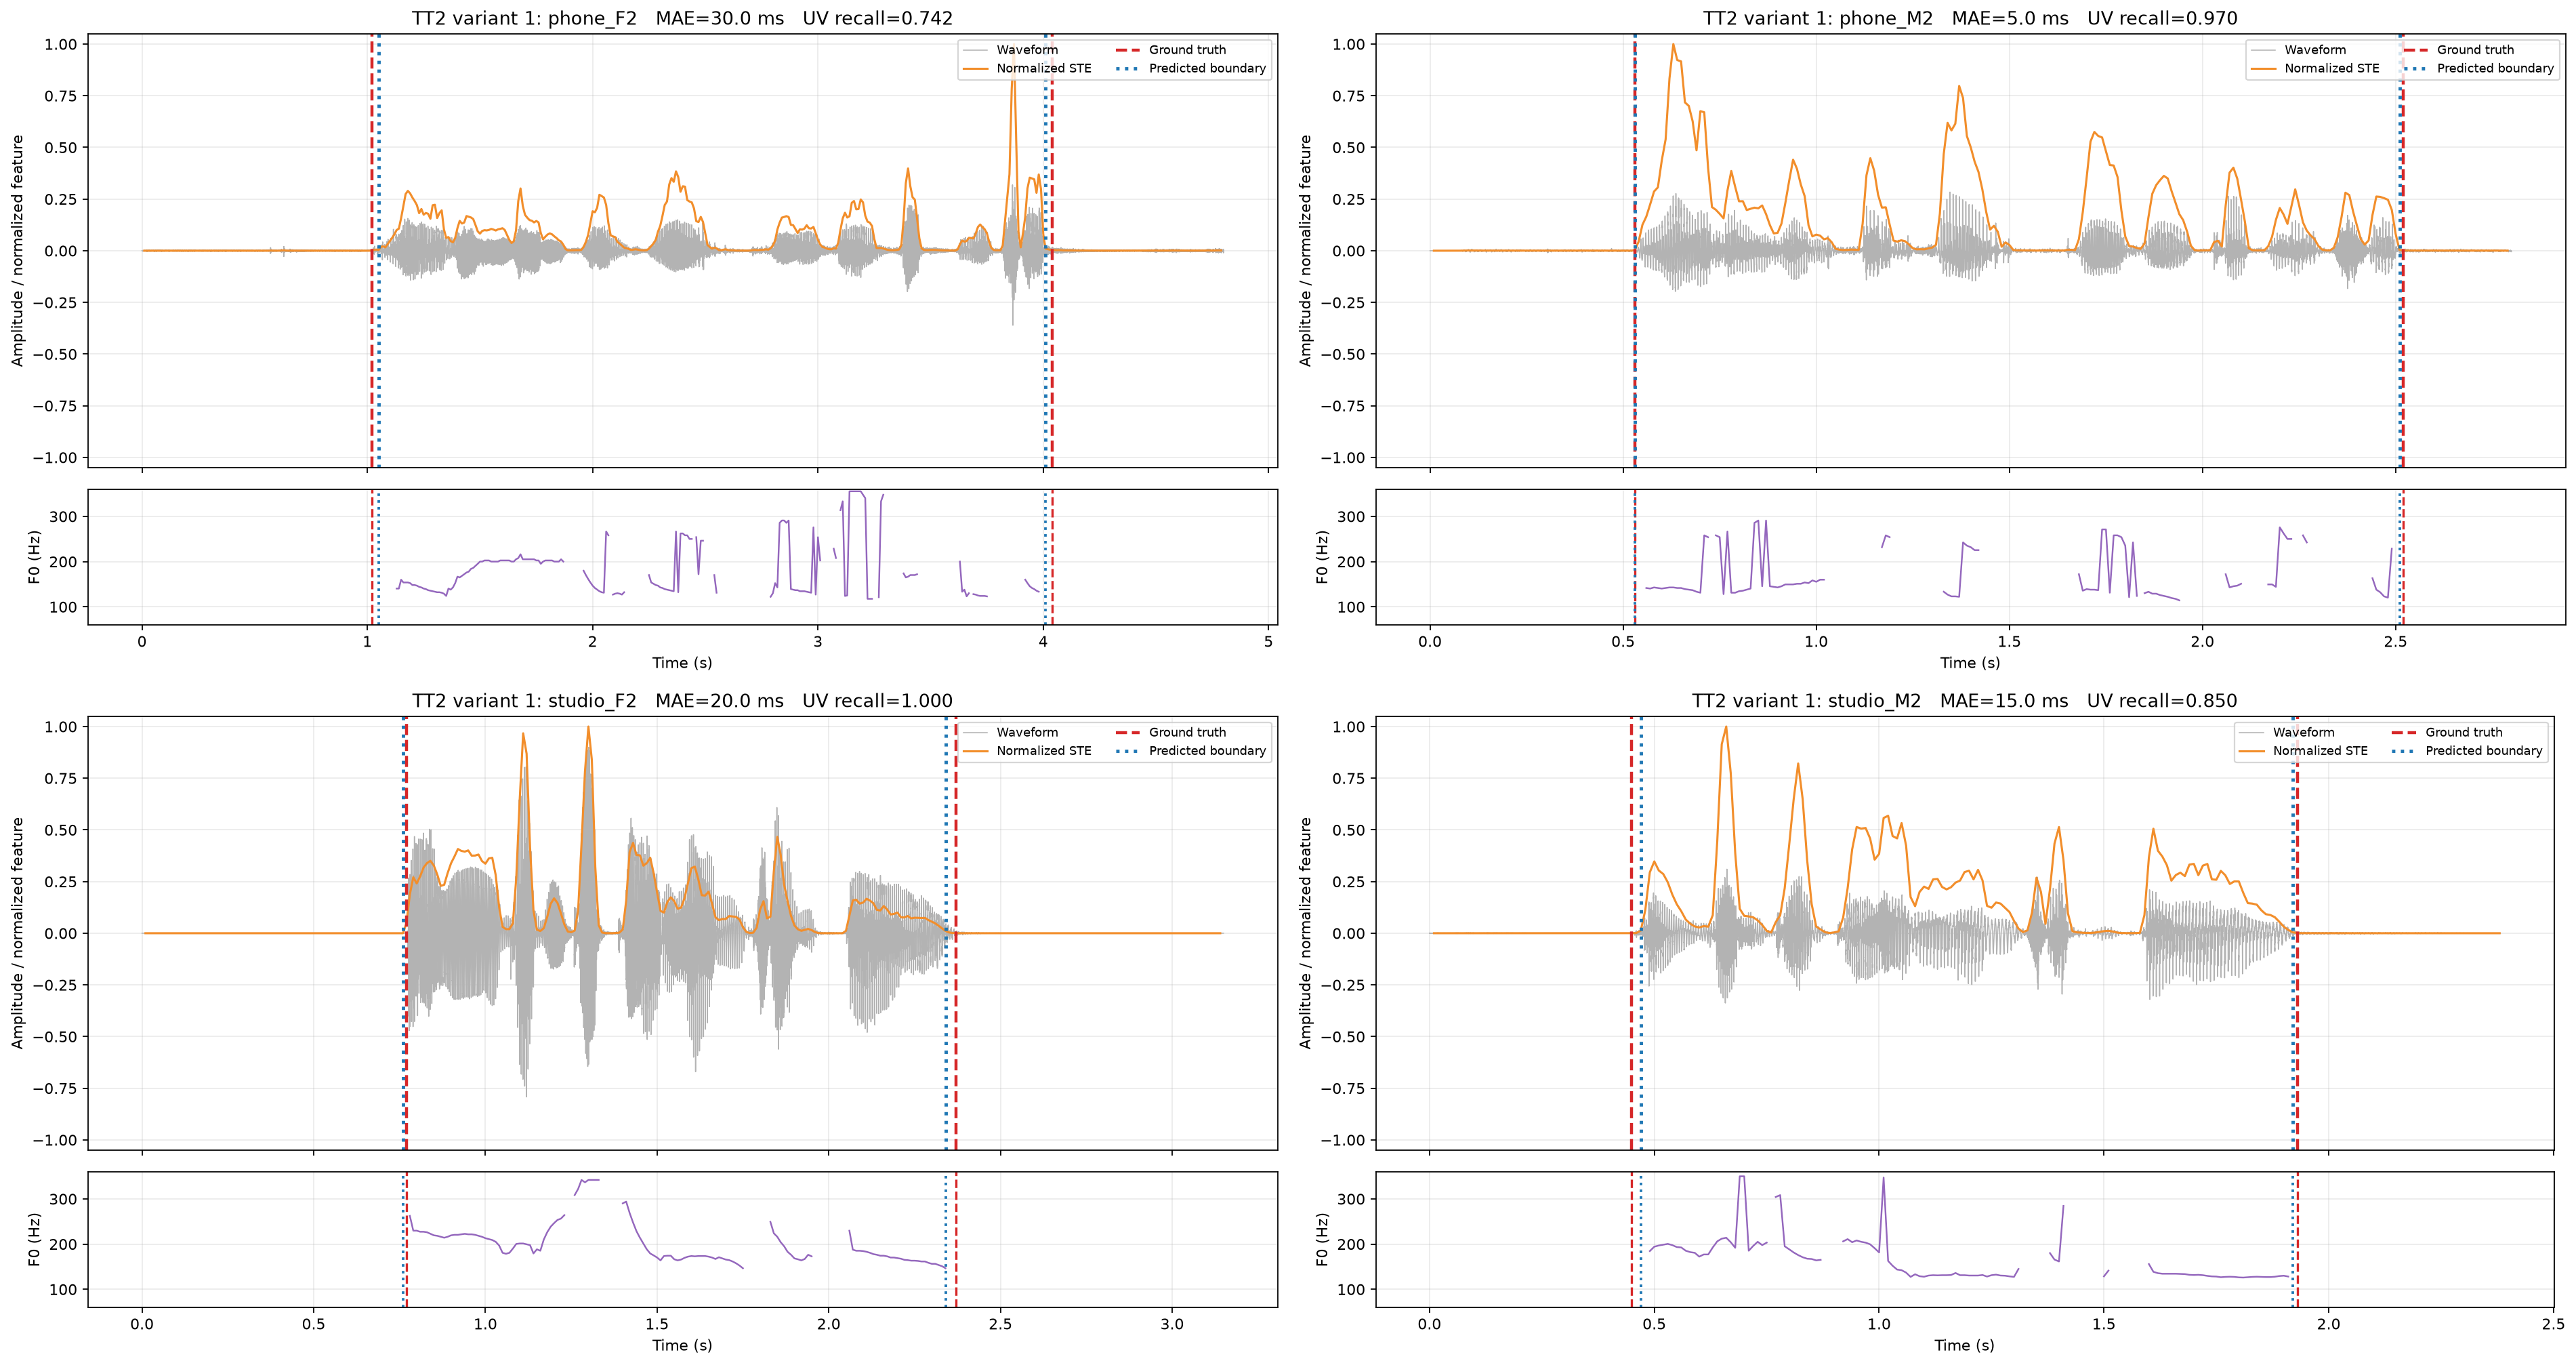
\includegraphics[width=\textwidth, height=4.6cm, keepaspectratio]{figures/tt2_composite.png}
      \end{tcolorbox}
    \end{column}

    \begin{column}{0.34\textwidth}
      \begin{tcolorbox}[mintcard]
        {\fontsize{9pt}{10pt}\selectfont\color{mintGreen}\textbf{Adaptability}}\\[2pt]
        {\fontsize{8pt}{9.5pt}\selectfont
        $\bullet$ Mean MAE: \textbf{17.50 ms} (20.00 ms ext)\\[2pt]
        $\bullet$ Fully unsupervised per utterance\\[2pt]
        $\bullet$ Excellent frame F1: \textbf{0.977 -- 0.988}}
      \end{tcolorbox}
      \vskip4pt
      \begin{tcolorbox}[warncard]
        {\fontsize{9pt}{10pt}\selectfont\color{amberWarn}\textbf{Truncation Bias}}\\[2pt]
        {\fontsize{8pt}{9.5pt}\selectfont
        $\bullet$ Weight $W=5$ raises threshold\\[2pt]
        $\bullet$ Truncates trailing unvoiced phonemes}
      \end{tcolorbox}
    \end{column}
  \end{columns}
\end{frame}

% ==============================================================================
% SLIDE 10: ALG 2 OPTIMIZATION
% ==============================================================================
\section{ALG 2 $\cdot$ OPTIMIZATION}
\begin{frame}
  \frametitle{Adaptive Weight $W$ Tuning for Studio Acoustics}
  \begin{columns}[T]
    \begin{column}{0.31\textwidth}
      \begin{tcolorbox}[glowcard]
        \centering
        {\fontsize{9.5pt}{11pt}\selectfont\color{cyanGlow}\textbf{HIGH NOISE ($W \uparrow$)}}\\[4pt]
        \raggedright{\fontsize{8.5pt}{10pt}\selectfont
        $\bullet$ Increase $W$ in noisy environments\\[3pt]
        $\bullet$ Raises threshold above noise floor\\[3pt]
        $\bullet$ Prevents false speech triggers}
      \end{tcolorbox}
    \end{column}

    \begin{column}{0.31\textwidth}
      \begin{tcolorbox}[mintcard]
        \centering
        {\fontsize{9.5pt}{11pt}\selectfont\color{mintGreen}\textbf{CLEAN STUDIO ($W \downarrow$)}}\\[4pt]
        \raggedright{\fontsize{8.5pt}{10pt}\selectfont
        $\bullet$ Decrease $W$ in clean recordings\\[3pt]
        $\bullet$ Pulls threshold toward silence\\[3pt]
        $\bullet$ Preserves weak unvoiced phonemes}
      \end{tcolorbox}
    \end{column}

    \begin{column}{0.31\textwidth}
      \begin{tcolorbox}[warncard]
        \centering
        {\fontsize{9.5pt}{11pt}\selectfont\color{amberWarn}\textbf{ENGINEERING VALUE}}\\[4pt]
        \raggedright{\fontsize{8.5pt}{10pt}\selectfont
        $\bullet$ Direct trade-off knob\\[3pt]
        $\bullet$ Noise rejection vs phoneme clipping\\[3pt]
        $\bullet$ No retraining required when SNR shifts}
      \end{tcolorbox}
    \end{column}
  \end{columns}
  
  \vspace{10pt}
  \begin{center}
    {\fontsize{8.5pt}{10pt}\selectfont\color{textMuted}\textbf{Key Takeaway:} Weight $W$ provides transparent control over noise sensitivity.}
  \end{center}
\end{frame}

% ==============================================================================
% SLIDE 11: STUDENT 3 COVER
% ==============================================================================
\section{STUDENT 3 $\cdot$ ALGORITHM 03}
\begin{frame}
  \frametitle{Parametric Gaussian Bayes Model}
  \begin{columns}[c]
    \begin{column}{0.62\textwidth}
      \begin{tcolorbox}[glowcard]
        {\fontsize{13pt}{15pt}\selectfont\color{cyanGlow}\textbf{Truong Bui Dien}}\\[3pt]
        {\fontsize{9.5pt}{11pt}\selectfont\color{textWhite}\textbf{Algorithm 03 $\cdot$ Statistical Bayes Separation}}\\[6pt]
        {\fontsize{8.5pt}{10pt}\selectfont\color{textMuted}
        $\bullet$ Reference: Classical Statistical Pattern Recognition\\[3pt]
        $\bullet$ Approach: Parametric Gaussian density estimation\\[3pt]
        $\bullet$ Training: Fit $\mu, \sigma$ for silence and speech frames\\[3pt]
        $\bullet$ Formulation: Analytical quadratic root at density intersection\\[3pt]
        $\bullet$ Advantage: Statistically grounded decision boundary}
      \end{tcolorbox}
    \end{column}

    \begin{column}{0.34\textwidth}
      \begin{center}
        \begin{tcolorbox}[portraitframe]
          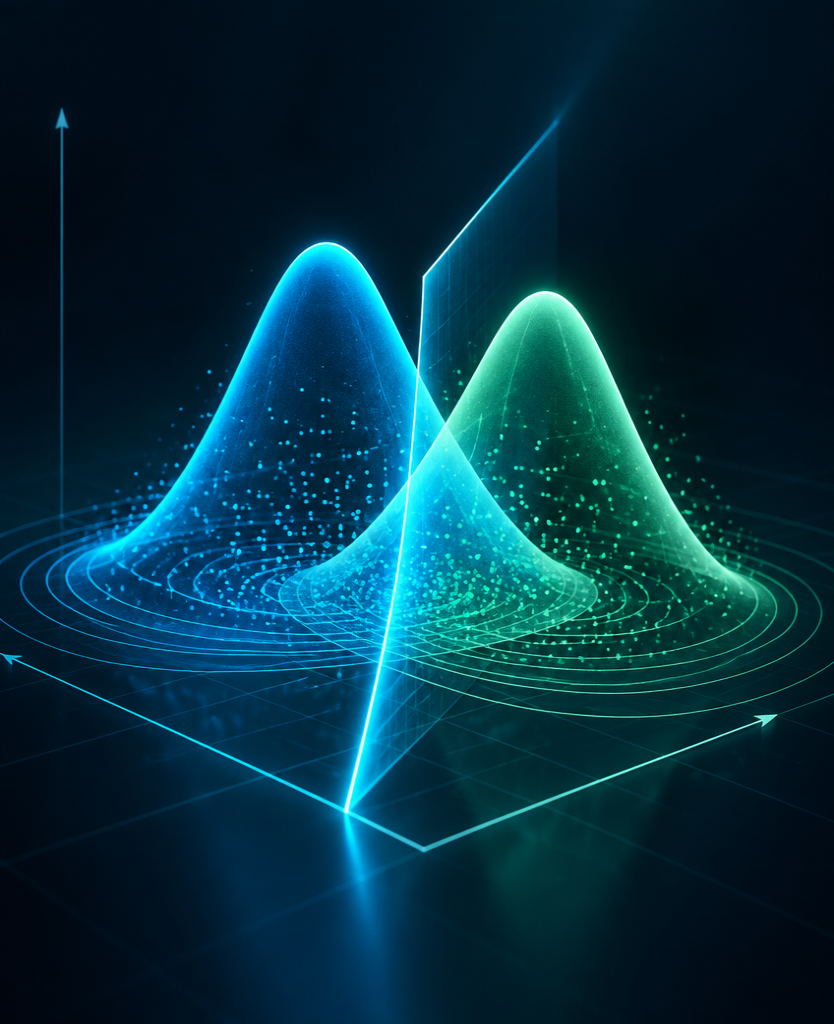
\includegraphics[width=\textwidth, height=4.2cm, keepaspectratio]{figures/student3_portrait.png}
        \end{tcolorbox}
      \end{center}
    \end{column}
  \end{columns}
\end{frame}

% ==============================================================================
% SLIDE 12: ALG 3 CORE METHOD
% ==============================================================================
\section{ALG 3 $\cdot$ CORE METHOD}
\begin{frame}
  \frametitle{From Empirical Statistics to Analytical Bayes Root}
  \begin{center}
    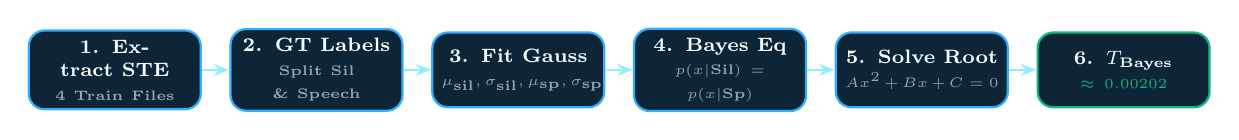
\begin{tikzpicture}[
      node distance=0.35cm,
      stepnode/.style={
        rectangle, rounded corners=2mm, fill=bgCard, draw=cyanAccent, line width=0.8pt,
        text=textWhite, align=center, font=\fontsize{7.5pt}{8.5pt}\selectfont\bfseries,
        minimum height=0.95cm, text width=1.95cm
      },
      flowarr/.style={-{Stealth[scale=0.75]}, draw=cyanGlow, line width=1pt}
    ]
      \node[stepnode] (b1) {1. Extract STE\\{\color{textMuted}\tiny 4 Train Files}};
      \node[stepnode, right=of b1] (b2) {2. GT Labels\\{\color{textMuted}\tiny Split Sil \& Speech}};
      \node[stepnode, right=of b2] (b3) {3. Fit Gauss\\{\color{textMuted}\tiny $\mu_{\text{sil}}, \sigma_{\text{sil}}, \mu_{\text{sp}}, \sigma_{\text{sp}}$}};
      \node[stepnode, right=of b3] (b4) {4. Bayes Eq\\{\color{textMuted}\tiny $p(x|\text{Sil})=p(x|\text{Sp})$}};
      \node[stepnode, right=of b4] (b5) {5. Solve Root\\{\color{textMuted}\tiny $A x^2 + B x + C = 0$}};
      \node[stepnode, right=of b5, draw=mintGreen] (b6) {6. $T_{\text{Bayes}}$\\{\color{mintGreen}\tiny $\approx 0.00202$}};

      \draw[flowarr] (b1) -- (b2);
      \draw[flowarr] (b2) -- (b3);
      \draw[flowarr] (b3) -- (b4);
      \draw[flowarr] (b4) -- (b5);
      \draw[flowarr] (b5) -- (b6);
    \end{tikzpicture}
  \end{center}

  \vspace{8pt}
  \begin{columns}[T]
    \begin{column}{0.48\textwidth}
      \begin{tcolorbox}[darkcard]
        {\fontsize{9pt}{10pt}\selectfont\color{cyanGlow}\textbf{Estimated Parameters from Train Set}}\\[3pt]
        {\fontsize{8.5pt}{10pt}\selectfont
        $\bullet$ Silence: $\mu_{\text{sil}} = 0.00033$, $\sigma_{\text{sil}} = 0.00047$\\[2pt]
        $\bullet$ Speech: $\mu_{\text{sp}} = 0.19652$, $\sigma_{\text{sp}} = 0.23327$\\[2pt]
        $\bullet$ Massive energy dynamic range separation}
      \end{tcolorbox}
    \end{column}

    \begin{column}{0.48\textwidth}
      \begin{tcolorbox}[mintcard]
        {\fontsize{9pt}{10pt}\selectfont\color{mintGreen}\textbf{Analytical Decision Root}}\\[3pt]
        {\fontsize{8.5pt}{10pt}\selectfont
        $\bullet$ Equiprobable intersection: $\mathbf{T_{\text{Bayes}} = 0.00202}$\\[2pt]
        $\bullet$ Closed-form analytical quadratic solution\\[2pt]
        $\bullet$ Post-processed with 200 ms minimum silence bridge}
      \end{tcolorbox}
    \end{column}
  \end{columns}
\end{frame}

% ==============================================================================
% SLIDE 13: ALG 3 EXPERIMENTS
% ==============================================================================
\section{ALG 3 $\cdot$ EXPERIMENTS}
\begin{frame}
  \frametitle{High Accuracy on Test Data (MAE = 11.25 ms)}
  \begin{columns}[c]
    \begin{column}{0.64\textwidth}
      \begin{tcolorbox}[whiteframe]
        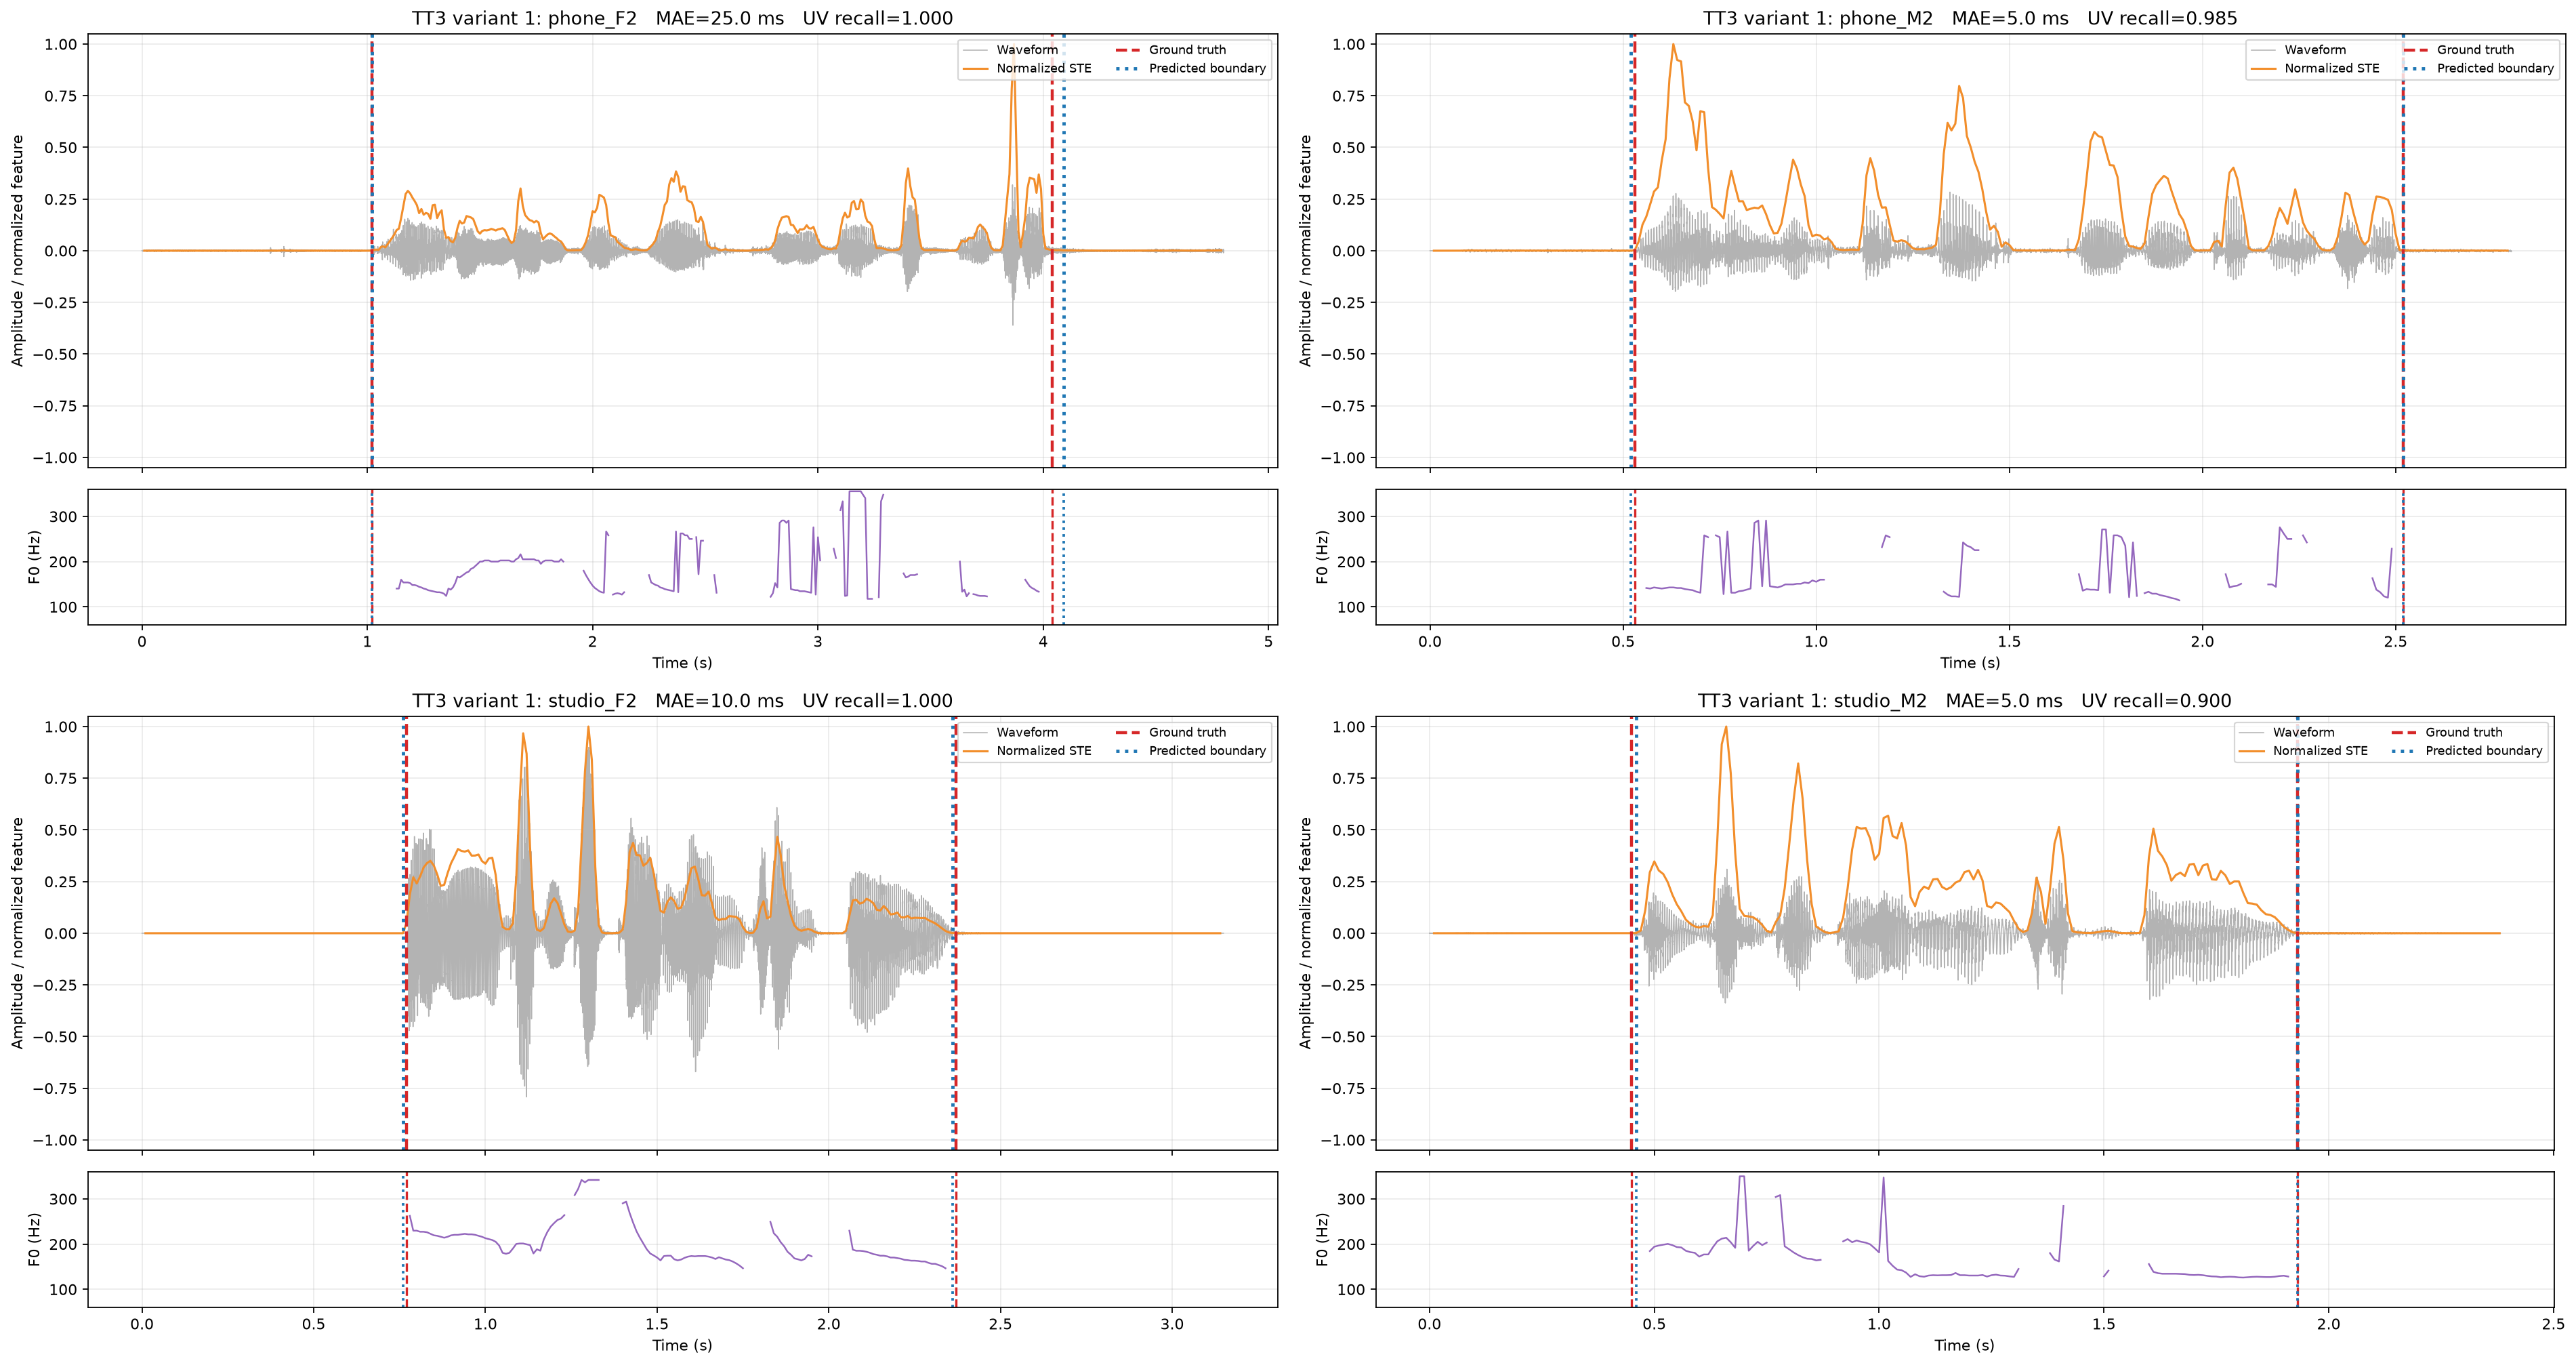
\includegraphics[width=\textwidth, height=4.6cm, keepaspectratio]{figures/tt3_composite.png}
      \end{tcolorbox}
    \end{column}

    \begin{column}{0.34\textwidth}
      \begin{tcolorbox}[mintcard]
        {\fontsize{9pt}{10pt}\selectfont\color{mintGreen}\textbf{Test Results}}\\[2pt]
        {\fontsize{8pt}{9.5pt}\selectfont
        $\bullet$ Mean MAE: \textbf{11.25 ms} (15.00 ms ext)\\[2pt]
        $\bullet$ High precision across studio audio\\[2pt]
        $\bullet$ Frame F1 score: \textbf{0.994}}
      \end{tcolorbox}
      \vskip4pt
      \begin{tcolorbox}[warncard]
        {\fontsize{9pt}{10pt}\selectfont\color{amberWarn}\textbf{Theoretical Critique}}\\[2pt]
        {\fontsize{8pt}{9.5pt}\selectfont
        $\bullet$ Energy is non-negative and skewed\\[2pt]
        $\bullet$ Gaussian assumption is flawed\\[2pt]
        $\bullet$ Works because cut is in low tail}
      \end{tcolorbox}
    \end{column}
  \end{columns}
\end{frame}

% ==============================================================================
% SLIDE 14: GROUP BENCHMARK (MANDATORY SUMMARY TABLE)
% ==============================================================================
\section{BENCHMARK $\cdot$ 4 TEST FILES}
\begin{frame}
  \frametitle{Quantitative Performance Comparison Across Algorithms}
  \begin{columns}[c]
    \begin{column}{0.55\textwidth}
      \begin{tcolorbox}[darkcard]
        \centering
        {\fontsize{8pt}{9.5pt}\selectfont\color{cyanGlow}\textbf{Summary Benchmark Table (4 Test Recordings)}}\\[3pt]
        \fontsize{6.8pt}{8.2pt}\selectfont
        \setlength{\tabcolsep}{3pt}
        \begin{tabularx}{\linewidth}{>{\raggedright\arraybackslash}Xcccc}
          \toprule
          \textbf{Method} & \textbf{MAE} & \textbf{RMSE} & \textbf{F1} & \textbf{UV} \\
          \midrule
          \textbf{TT1-1 (Hodgkinson)} & 8.75 & 11.34 & 0.993 & 0.971 \\
          \textbf{TT1-2 (DSP Classifier)} & \textbf{6.25} & \textbf{7.80} & \textbf{0.996} & 0.968 \\
          \midrule
          \textbf{TT2-1 (1D Histogram)} & 17.50 & 18.81 & 0.977 & 0.891 \\
          \textbf{TT2-2 (Joint STE-ZCR)} & 20.00 & 21.56 & 0.988 & \textbf{0.947} \\
          \midrule
          \textbf{TT3-1 (1D Gaussian)} & 11.25 & 14.87 & 0.994 & 0.971 \\
          \textbf{TT3-2 (Multivariate)} & 15.00 & 16.34 & 0.978 & 0.903 \\
          \bottomrule
        \end{tabularx}
      \end{tcolorbox}
      \vspace{2pt}
      \begin{tcolorbox}[mintcard]
        {\fontsize{7.5pt}{8.5pt}\selectfont\color{mintGreen}\textbf{Key Finding:} TT1-2 achieves lowest boundary error (6.25 ms MAE). TT2-2 achieves highest unvoiced phoneme recall (94.7\%).}
      \end{tcolorbox}
    \end{column}

    \begin{column}{0.43\textwidth}
      \begin{tcolorbox}[whiteframe]
        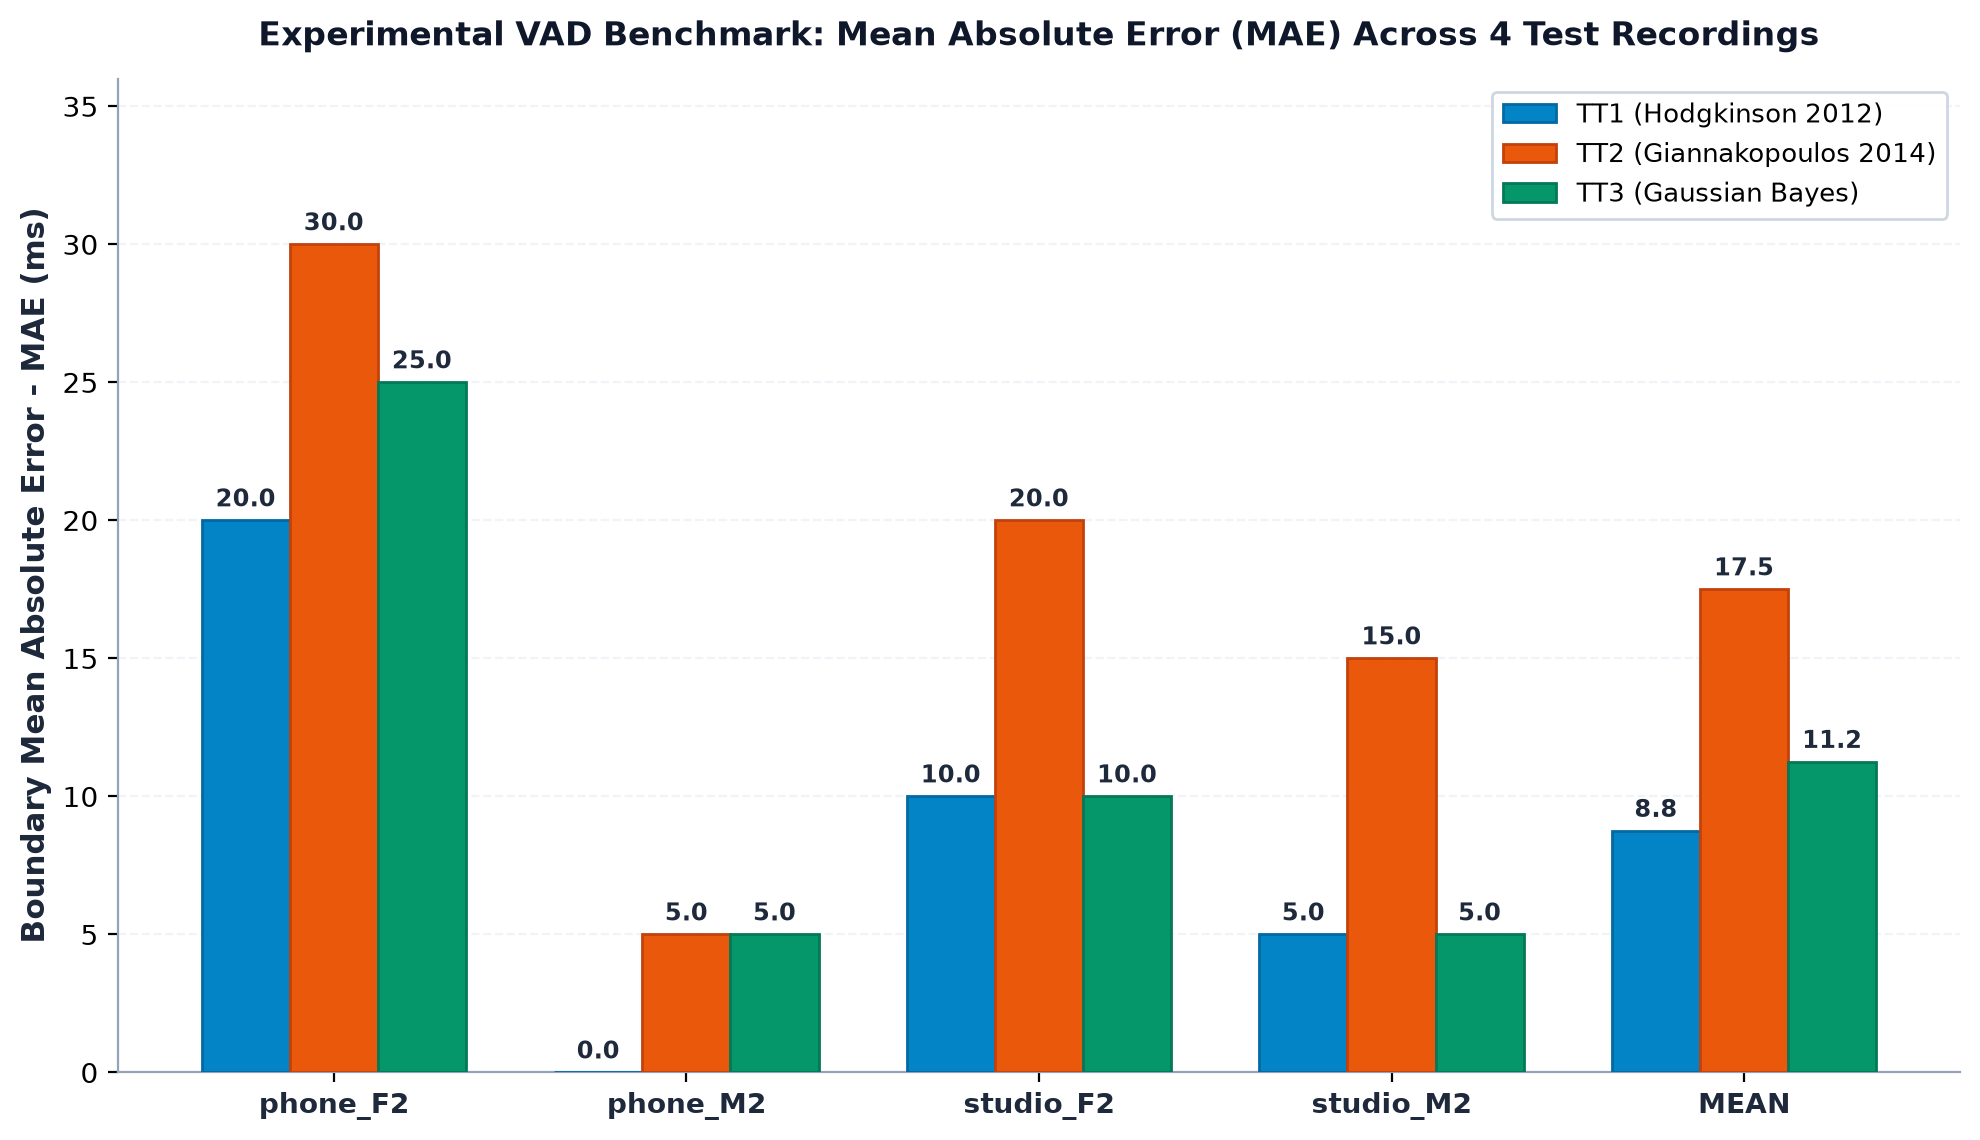
\includegraphics[width=\textwidth, height=4.5cm, keepaspectratio]{figures/benchmark_plot.png}
      \end{tcolorbox}
    \end{column}
  \end{columns}
\end{frame}

% ==============================================================================
% SLIDE 15: LIVE DEMO PROTOCOL
% ==============================================================================
\section{LIVE DEMO PROTOCOL}
\begin{frame}
  \frametitle{Four-Quadrant Display on Teacher Laptop}
  \begin{columns}[T]
    \begin{column}{0.24\textwidth}
      \begin{tcolorbox}[darkcard]
        \centering
        {\fontsize{9pt}{10pt}\selectfont\color{cyanGlow}\textbf{01 $\cdot$ INPUT}}\\[3pt]
        \raggedright{\fontsize{7.5pt}{9pt}\selectfont
        $\bullet$ 4 test WAV files\\[2pt]
        $\bullet$ Ground-truth .lab\\[2pt]
        $\bullet$ No audio upload}
      \end{tcolorbox}
    \end{column}

    \begin{column}{0.24\textwidth}
      \begin{tcolorbox}[darkcard]
        \centering
        {\fontsize{9pt}{10pt}\selectfont\color{cyanGlow}\textbf{02 $\cdot$ ENV}}\\[3pt]
        \raggedright{\fontsize{7.5pt}{9pt}\selectfont
        $\bullet$ Local venv via uv\\[2pt]
        $\bullet$ Python 3.12+\\[2pt]
        $\bullet$ Built-in numpy}
      \end{tcolorbox}
    \end{column}

    \begin{column}{0.24\textwidth}
      \begin{tcolorbox}[darkcard]
        \centering
        {\fontsize{9pt}{10pt}\selectfont\color{cyanGlow}\textbf{03 $\cdot$ NOTEBOOKS}}\\[3pt]
        \raggedright{\fontsize{7.5pt}{9pt}\selectfont
        $\bullet$ Individual .ipynb\\[2pt]
        $\bullet$ Pre-run outputs\\[2pt]
        $\bullet$ Zero demo delay}
      \end{tcolorbox}
    \end{column}

    \begin{column}{0.24\textwidth}
      \begin{tcolorbox}[mintcard]
        \centering
        {\fontsize{9pt}{10pt}\selectfont\color{mintGreen}\textbf{04 $\cdot$ QUADRANT}}\\[3pt]
        \raggedright{\fontsize{7.5pt}{9pt}\selectfont
        $\bullet$ 4 figures tiled\\[2pt]
        $\bullet$ 4 screen corners\\[2pt]
        $\bullet$ metrics.json ready}
      \end{tcolorbox}
    \end{column}
  \end{columns}

  \vspace{10pt}
  \begin{tcolorbox}[glowcard]
    {\fontsize{8.5pt}{10pt}\selectfont\color{cyanGlow}\textbf{Submission Protocol:}}
    {\fontsize{8pt}{9.5pt}\selectfont
    Directory \texttt{03-Phan-doan-tin-hieu-tieng-noi-khoang-lang} containing group PDF slide + individual notebooks. Audio files strictly excluded as required.}
  \end{tcolorbox}
\end{frame}

% ==============================================================================
% SLIDE 16: CONCLUSION
% ==============================================================================
\section{CONCLUSION $\cdot$ GROUP 03}
\begin{frame}
  \frametitle{Key Takeaways \& Q\&A Session}
  \begin{columns}[T]
    \begin{column}{0.31\textwidth}
      \begin{tcolorbox}[mintcard]
        \centering
        {\fontsize{9.5pt}{11pt}\selectfont\color{mintGreen}\textbf{ENERGY BASELINE}}\\[4pt]
        \raggedright{\fontsize{8.5pt}{10pt}\selectfont
        $\bullet$ Normalized STE is a strong foundation\\[3pt]
        $\bullet$ Clean studio error is only 5--10 ms\\[3pt]
        $\bullet$ Captures dominant speech boundaries}
      \end{tcolorbox}
    \end{column}

    \begin{column}{0.31\textwidth}
      \begin{tcolorbox}[glowcard]
        \centering
        {\fontsize{9.5pt}{11pt}\selectfont\color{cyanGlow}\textbf{UNVOICED SOUNDS}}\\[4pt]
        \raggedright{\fontsize{8.5pt}{10pt}\selectfont
        $\bullet$ Weak energy mimics background noise\\[3pt]
        $\bullet$ ZCR \& pre-emphasis aid discrimination\\[3pt]
        $\bullet$ Energy floor prevents noise false alarms}
      \end{tcolorbox}
    \end{column}

    \begin{column}{0.31\textwidth}
      \begin{tcolorbox}[warncard]
        \centering
        {\fontsize{9.5pt}{11pt}\selectfont\color{amberWarn}\textbf{MODEL COMPLEXITY}}\\[4pt]
        \raggedright{\fontsize{8.5pt}{10pt}\selectfont
        $\bullet$ 4 training files = small sample size\\[3pt]
        $\bullet$ Simple models generalize better\\[3pt]
        $\bullet$ 1D Gaussian beats 4D full covariance}
      \end{tcolorbox}
    \end{column}
  \end{columns}

  \vspace{12pt}
  \begin{center}
    {\fontsize{13pt}{15pt}\selectfont\color{cyanGlow}\textbf{Thank You for Your Attention!}}\\[4pt]
    {\fontsize{9pt}{10pt}\selectfont\color{textWhite}\textbf{Questions \& Answers Session}}
  \end{center}
\end{frame}

% ==============================================================================
% SLIDE 17: APPENDIX 01 - PREPROCESSING
% ==============================================================================
\section{APPENDIX 01 $\cdot$ PREPROCESSING}
\begin{frame}
  \frametitle{Standard Parameters \& 200 ms Silence Bridging}
  \begin{columns}[c]
    \begin{column}{0.58\textwidth}
      \begin{tcolorbox}[whiteframe]
        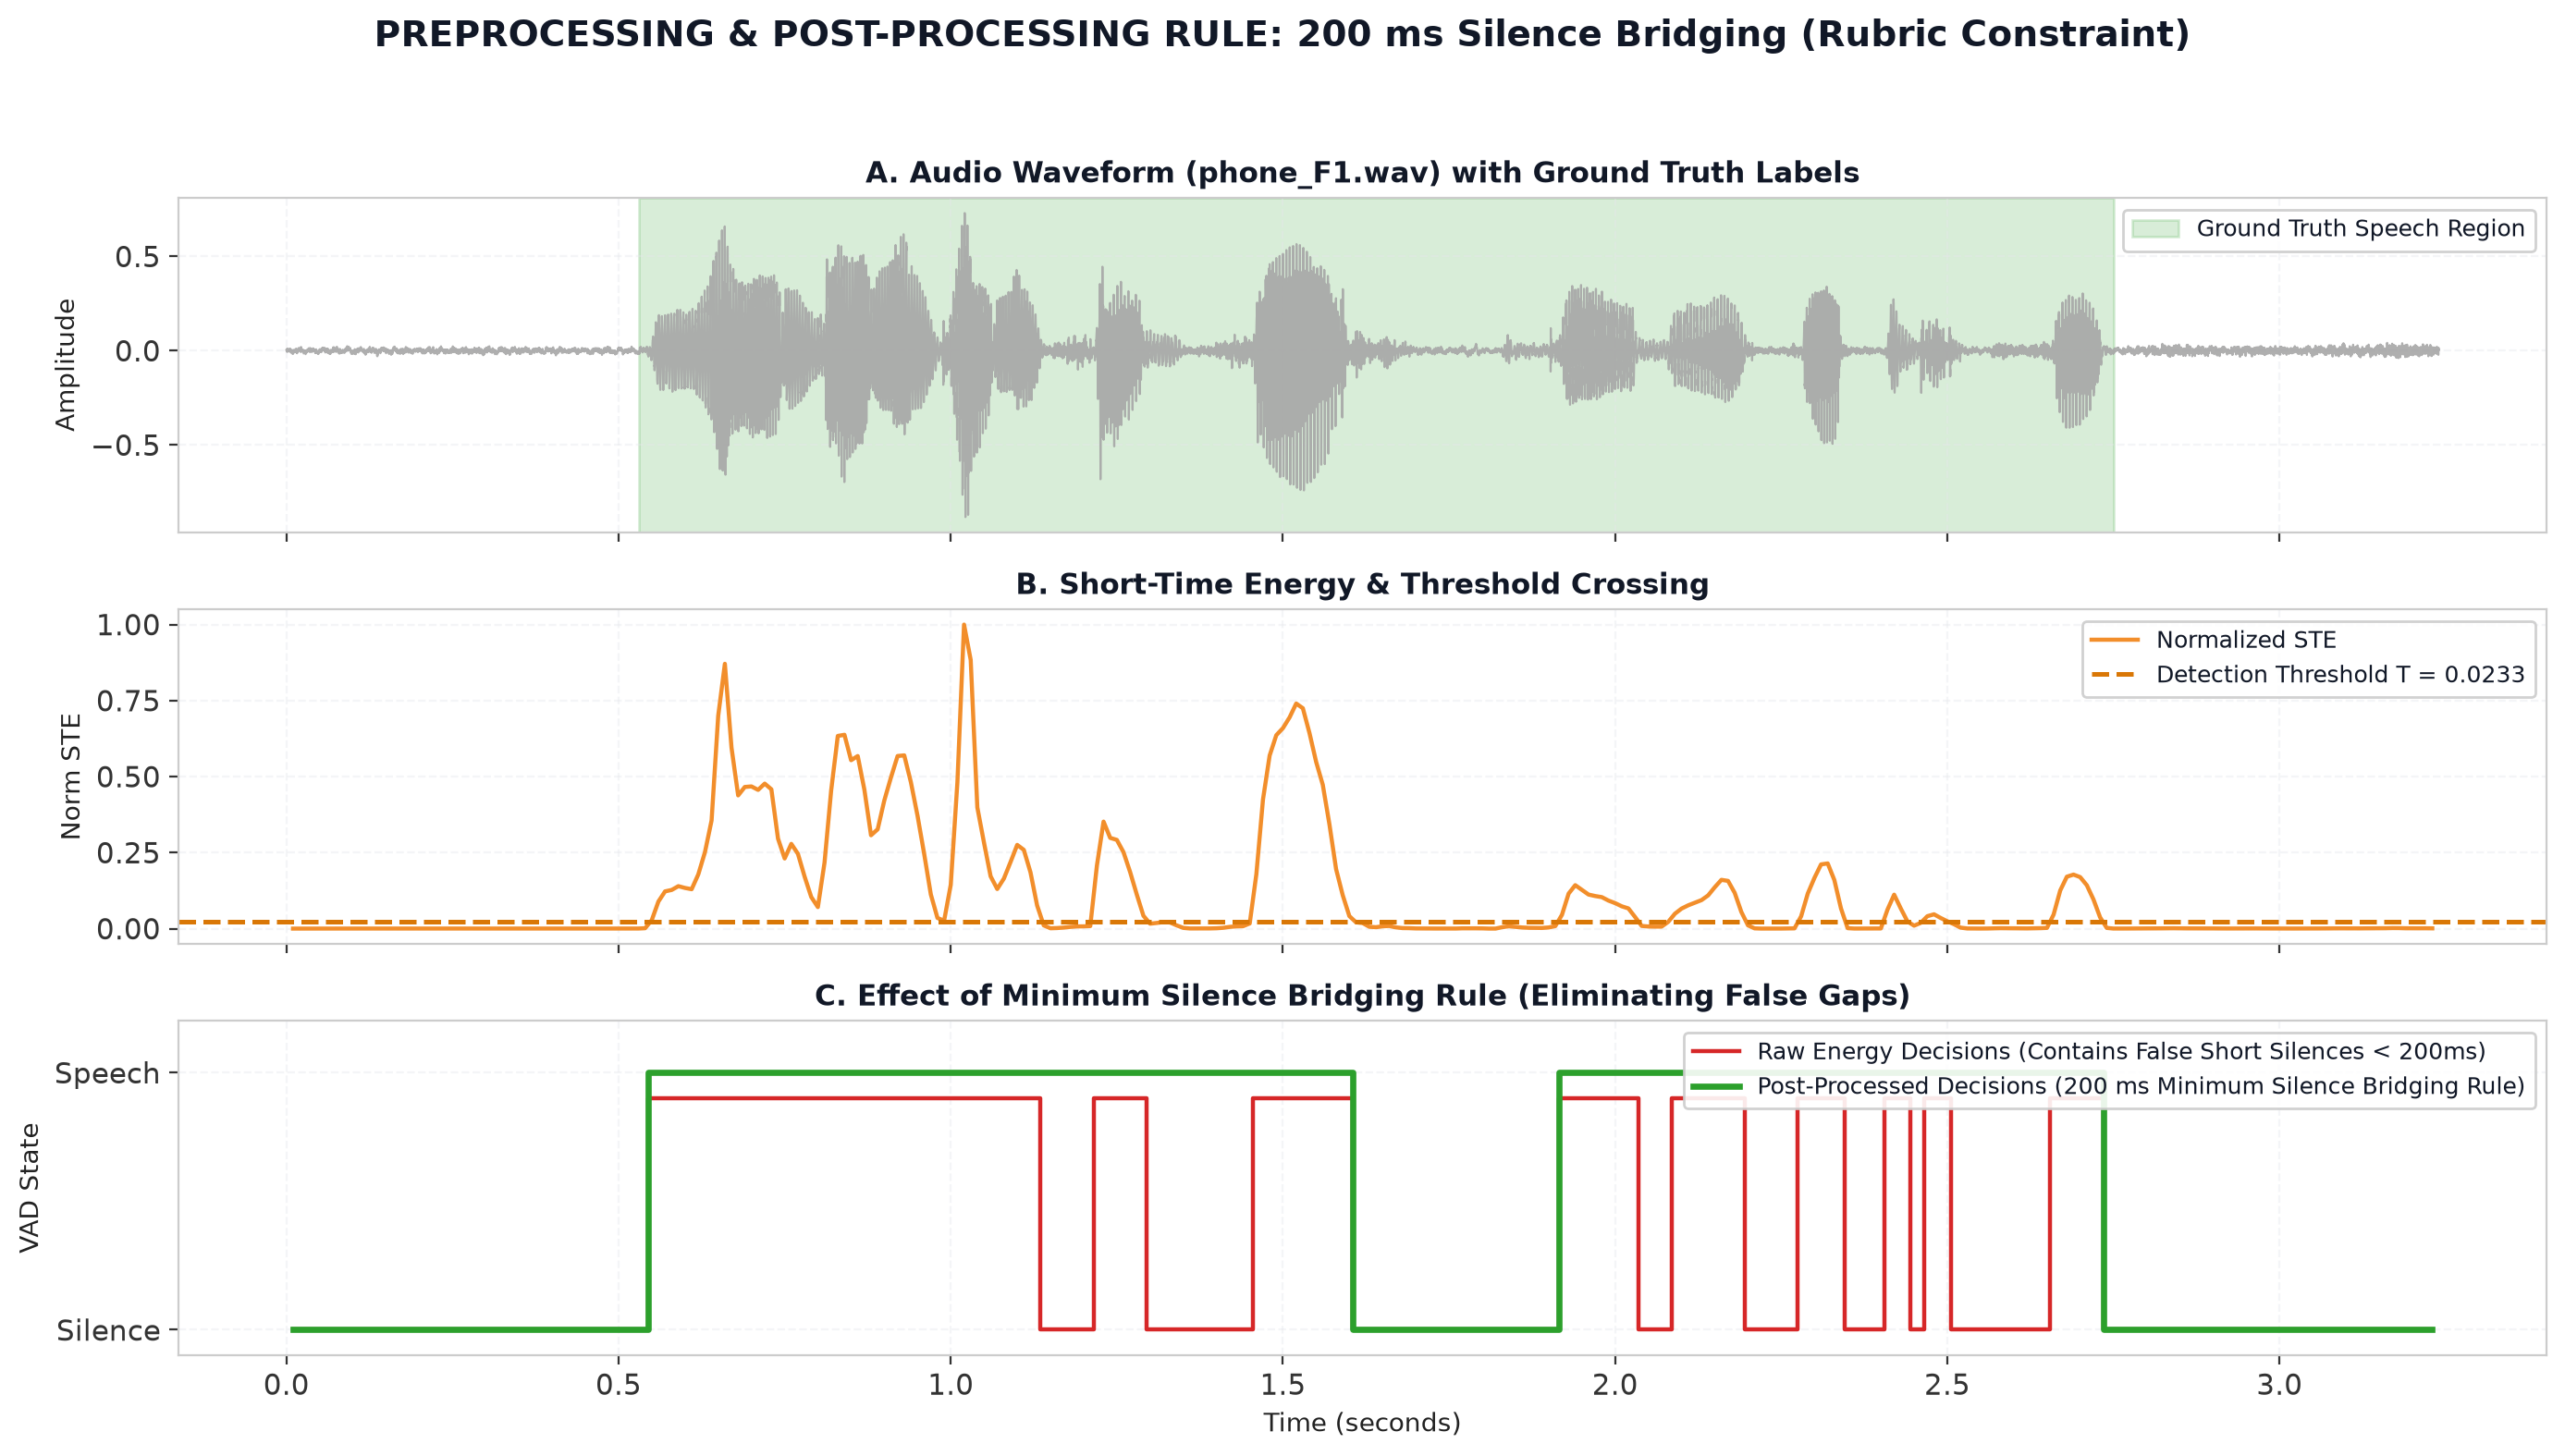
\includegraphics[width=\textwidth, height=4.6cm, keepaspectratio]{figures/preprocessing_bridge.png}
      \end{tcolorbox}
    \end{column}

    \begin{column}{0.40\textwidth}
      \begin{tcolorbox}[darkcard]
        {\fontsize{8.5pt}{9.5pt}\selectfont\color{cyanGlow}\textbf{DSP Hyperparameters}}\\[2pt]
        {\fontsize{7.5pt}{9pt}\selectfont
        $\bullet$ $F_s = 16\text{ kHz}$ (speech standard bandwidth)\\[2pt]
        $\bullet$ Frame: 25 ms (400 samples, quasi-stationary)\\[2pt]
        $\bullet$ Hop: 10 ms (160 samples, 60\% overlap grid)\\[2pt]
        $\bullet$ STE norm: $E_m / \max_k(E_k) \in [0, 1]$}
      \end{tcolorbox}
      \vskip3pt
      \begin{tcolorbox}[mintcard]
        {\fontsize{8.5pt}{9.5pt}\selectfont\color{mintGreen}\textbf{Bridging Invariant}}\\[2pt]
        {\fontsize{7.5pt}{9pt}\selectfont
        $\bullet$ Silence $< 200\text{ ms}$ is bridged (rule)\\[2pt]
        $\bullet$ Speech $< 50\text{ ms}$ is dropped (click noise)}
      \end{tcolorbox}
    \end{column}
  \end{columns}
\end{frame}

% ==============================================================================
% SLIDE 18: APPENDIX 02 - TT1 TRAINING
% ==============================================================================
\section{APPENDIX 02 $\cdot$ TT1 TRAINING}
\begin{frame}
  \frametitle{Binary Search Optimization Convergence (40 Iterations)}
  \begin{columns}[c]
    \begin{column}{0.64\textwidth}
      \begin{tcolorbox}[whiteframe]
        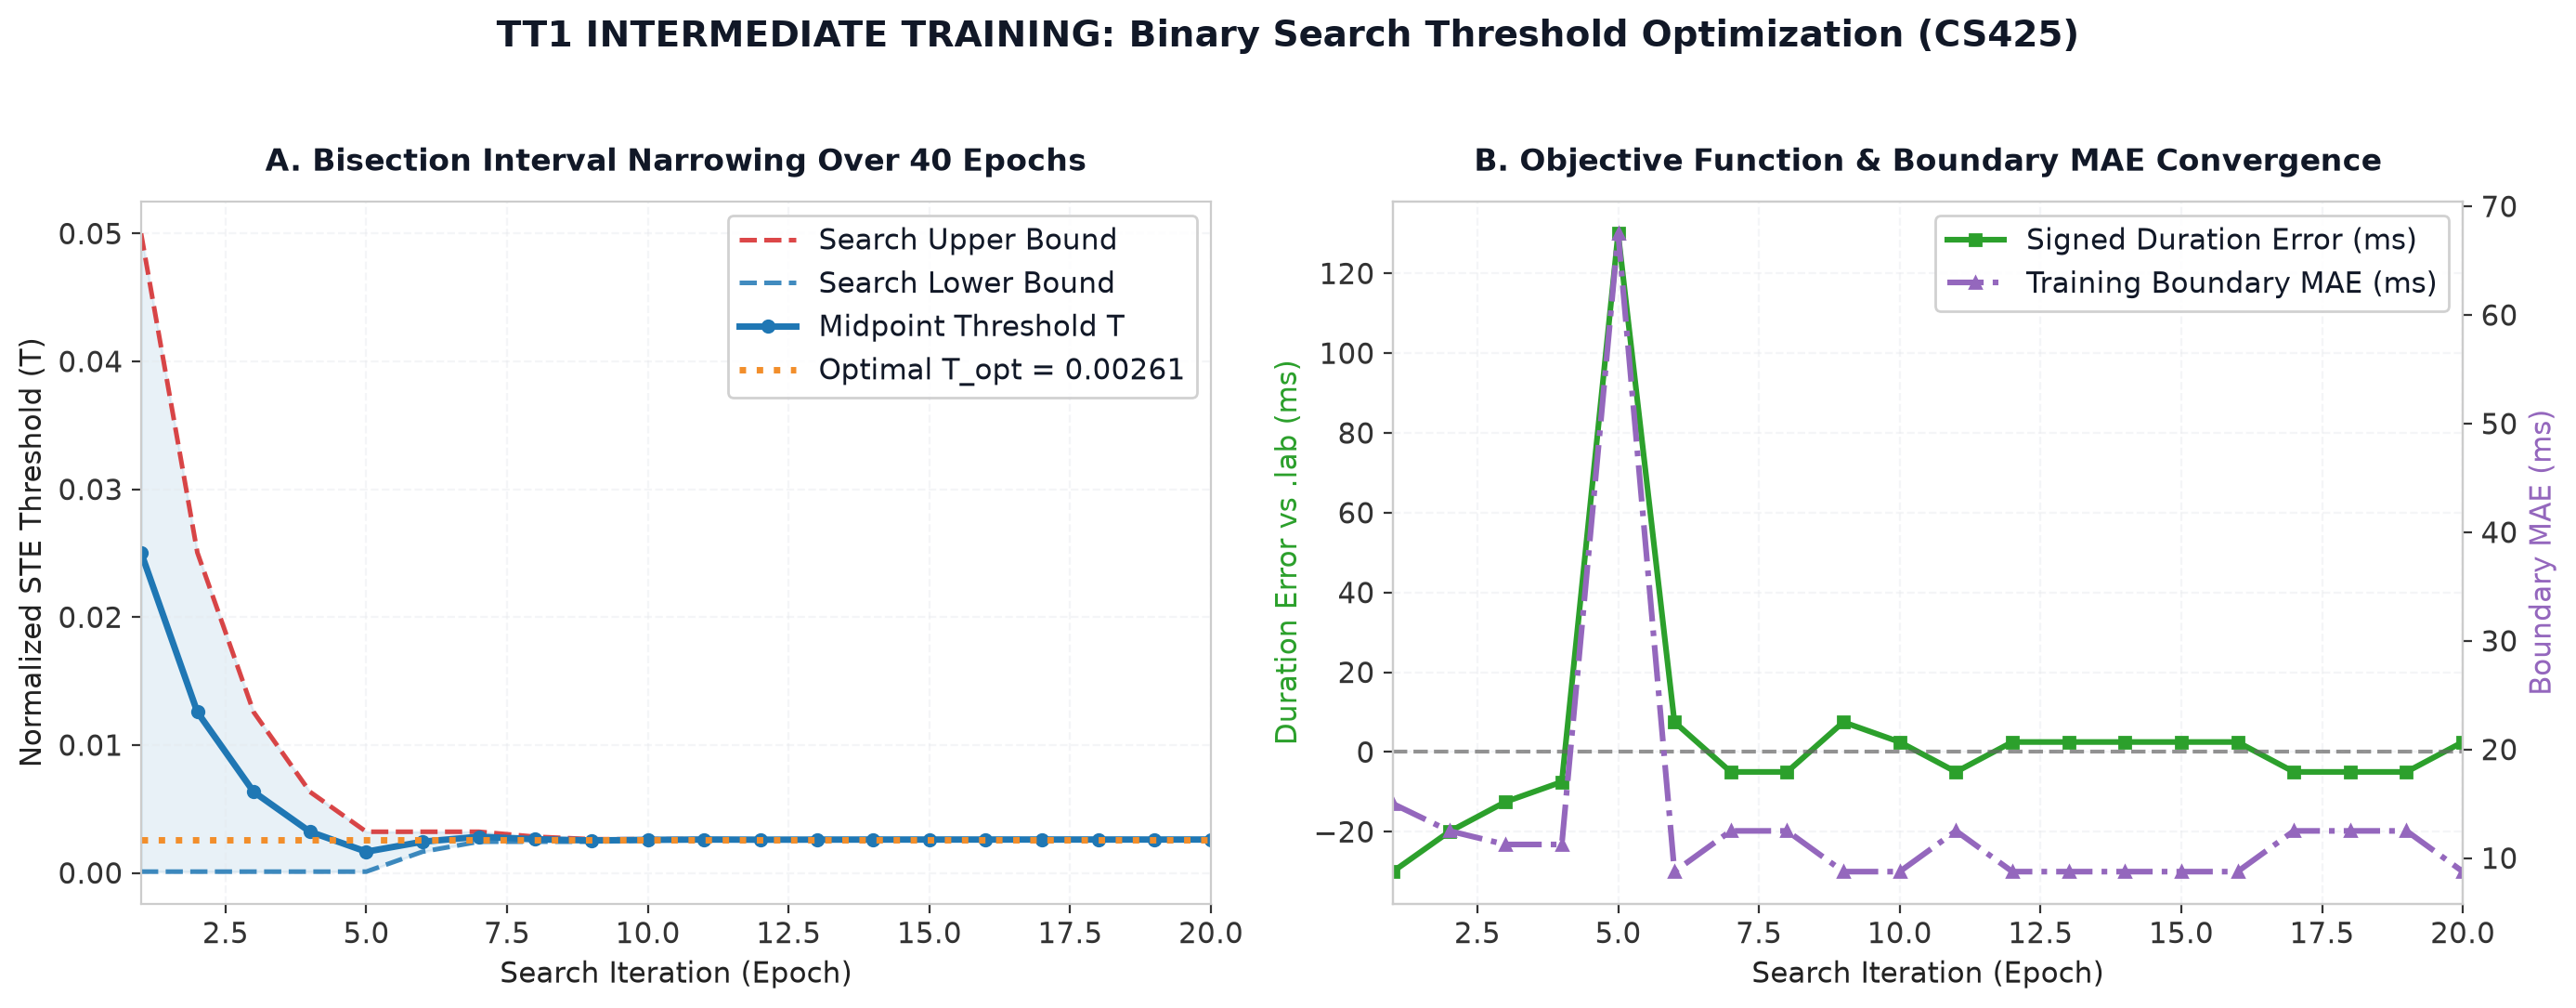
\includegraphics[width=\textwidth, height=4.6cm, keepaspectratio]{figures/tt1_train_convergence.png}
      \end{tcolorbox}
    \end{column}

    \begin{column}{0.34\textwidth}
      \begin{tcolorbox}[glowcard]
        {\fontsize{8.5pt}{9.5pt}\selectfont\color{cyanGlow}\textbf{Convergence Proof}}\\[2pt]
        {\fontsize{7.5pt}{9pt}\selectfont
        $\bullet$ Monotonic loss reduction\\[2pt]
        $\bullet$ Duration error balances to zero\\[2pt]
        $\bullet$ Converged: $\mathbf{T_{\text{opt}} = 0.00261}$\\[2pt]
        $\bullet$ Stable across all 4 train files}
      \end{tcolorbox}
    \end{column}
  \end{columns}
\end{frame}

% ==============================================================================
% SLIDE 19: APPENDIX 03 - TT2 TRAINING
% ==============================================================================
\section{APPENDIX 03 $\cdot$ TT2 TRAINING}
\begin{frame}
  \frametitle{Dual-Peak STE Histograms Across 4 Training Signals}
  \begin{columns}[c]
    \begin{column}{0.64\textwidth}
      \begin{tcolorbox}[whiteframe]
        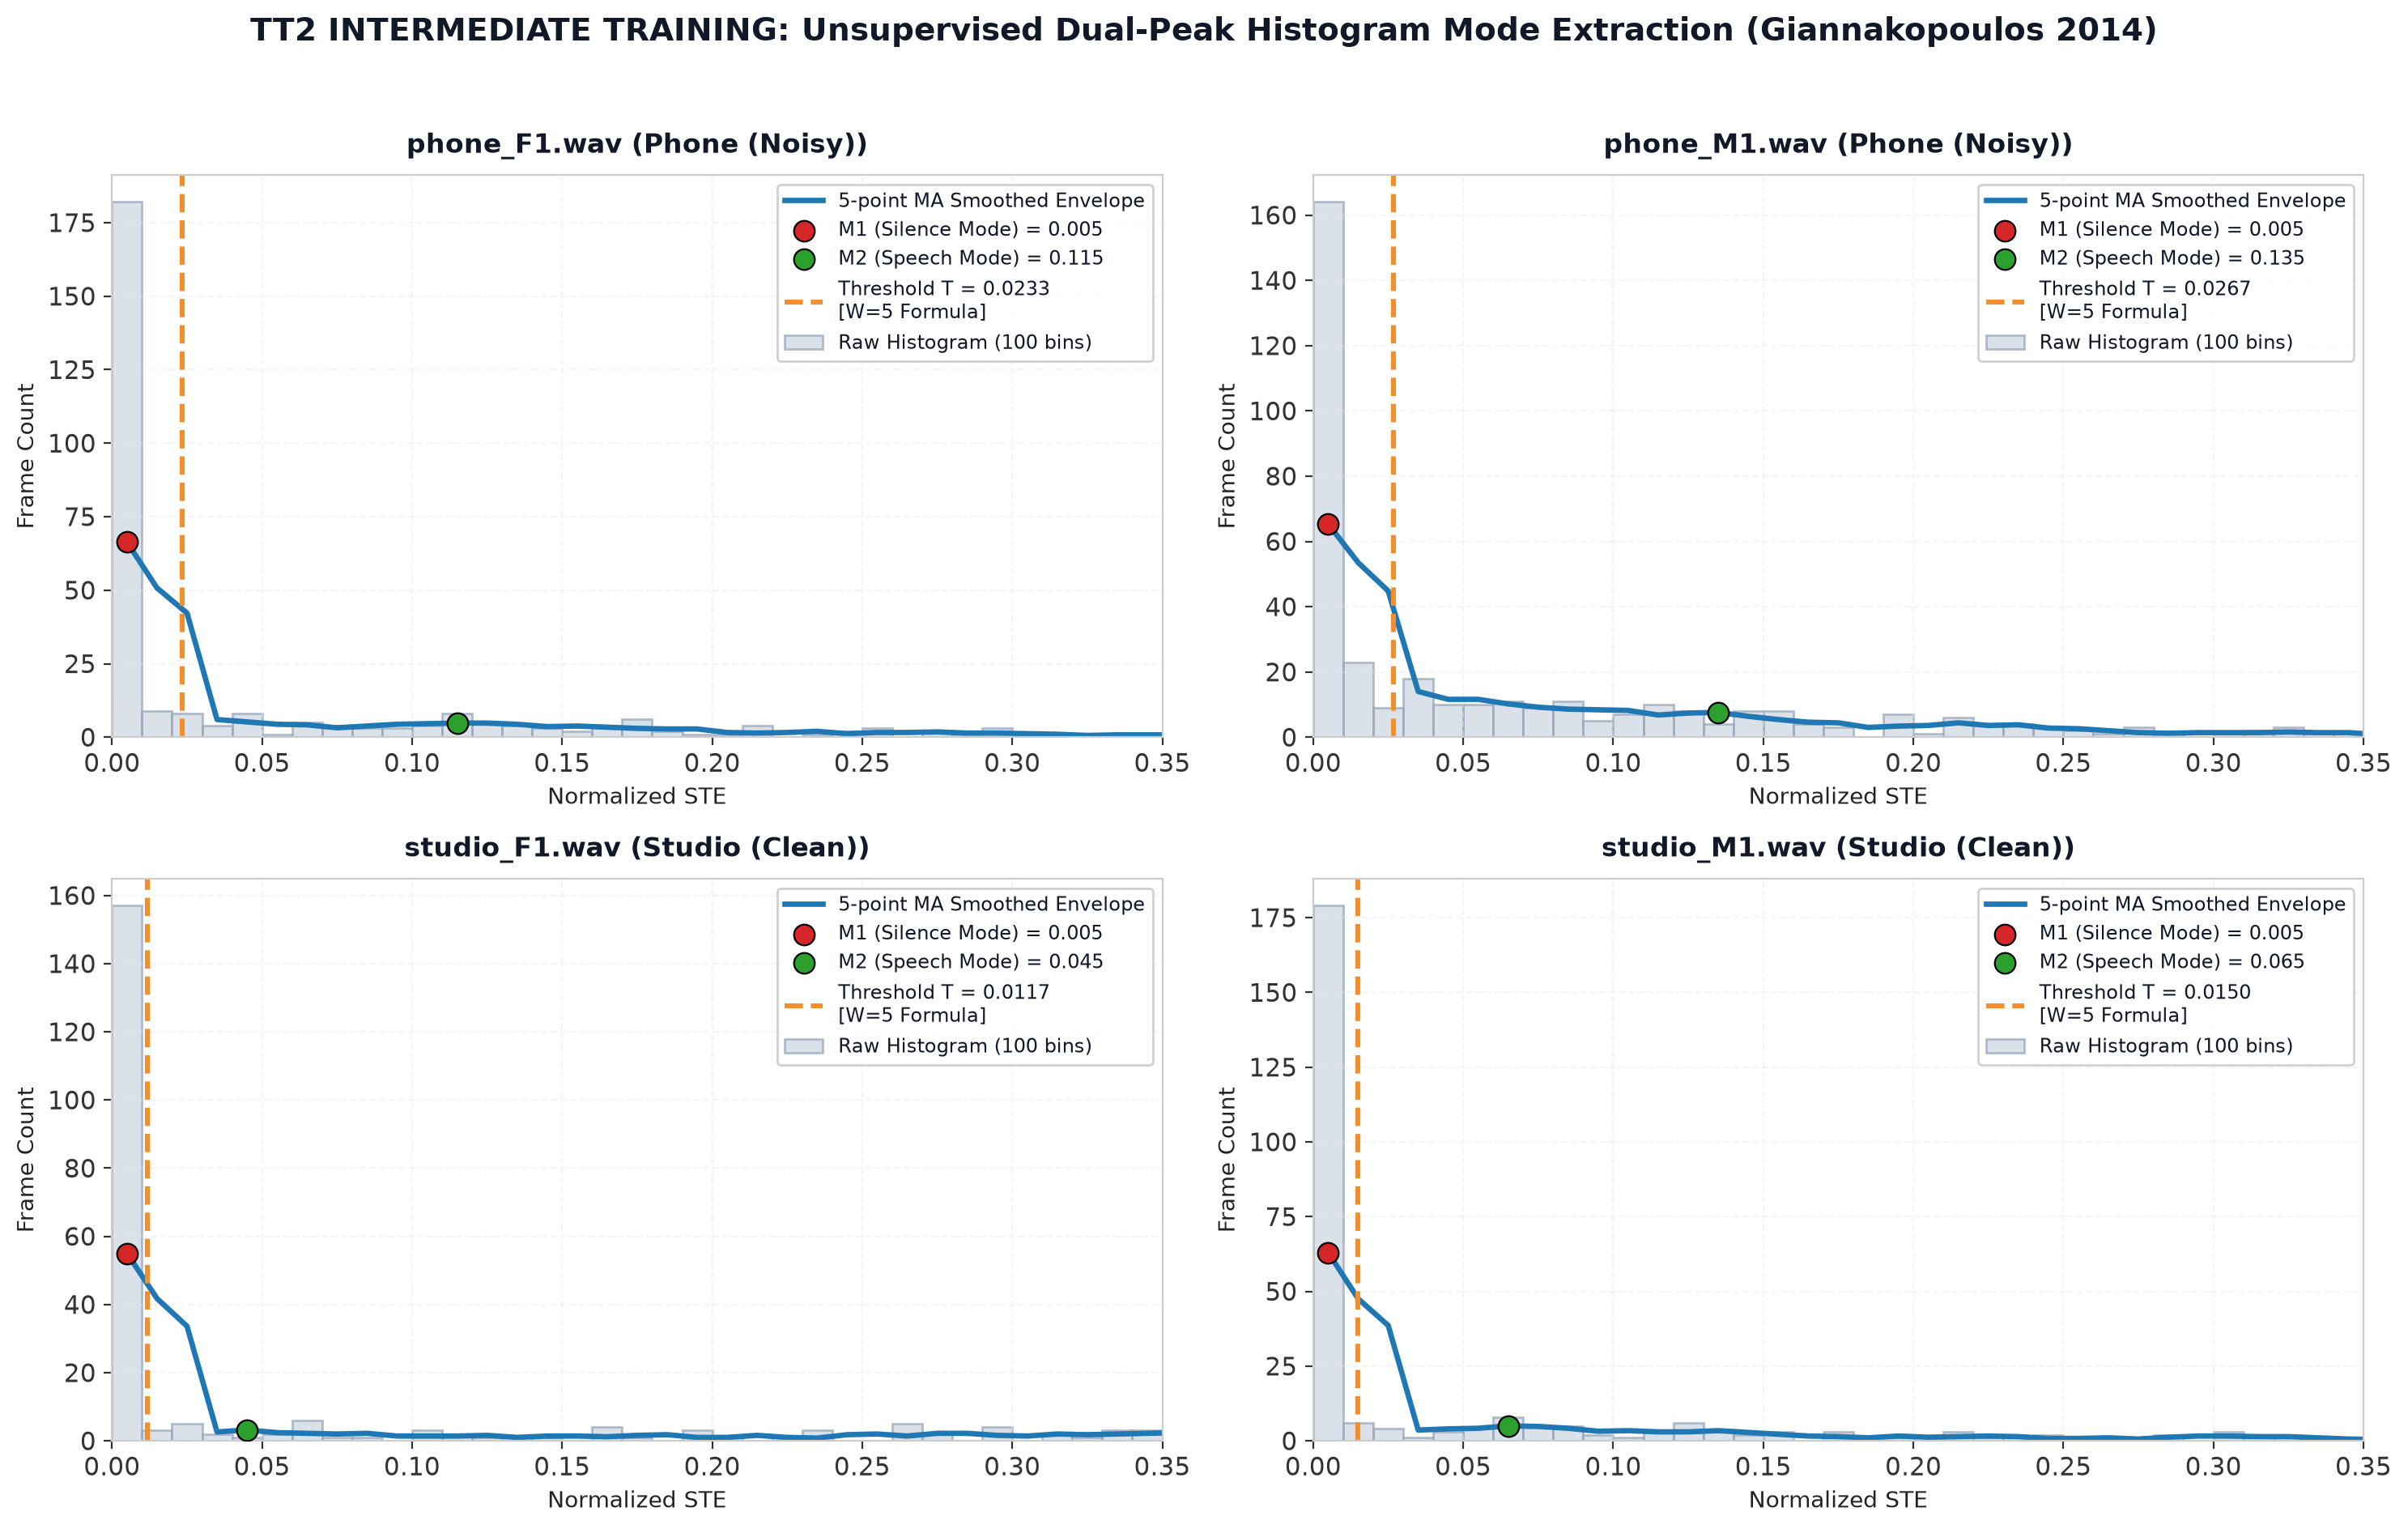
\includegraphics[width=\textwidth, height=4.6cm, keepaspectratio]{figures/tt2_train_histogram.png}
      \end{tcolorbox}
    \end{column}

    \begin{column}{0.34\textwidth}
      \begin{tcolorbox}[glowcard]
        {\fontsize{8.5pt}{9.5pt}\selectfont\color{cyanGlow}\textbf{Histogram Insights}}\\[2pt]
        {\fontsize{7.5pt}{9pt}\selectfont
        $\bullet$ 100 bins capture energy range\\[2pt]
        $\bullet$ 5-point MA filter removes noise\\[2pt]
        $\bullet$ Clear mode separation:\\[2pt]
        $\quad M_1$ (silence) vs $M_2$ (speech)\\[2pt]
        $\bullet$ Unsupervised threshold placement}
      \end{tcolorbox}
    \end{column}
  \end{columns}
\end{frame}

% ==============================================================================
% SLIDE 20: APPENDIX 04 - TT3 TRAINING
% ==============================================================================
\section{APPENDIX 04 $\cdot$ TT3 TRAINING}
\begin{frame}
  \frametitle{Parametric Gaussian Modeling \& Bayes Separation}
  \begin{columns}[c]
    \begin{column}{0.64\textwidth}
      \begin{tcolorbox}[whiteframe]
        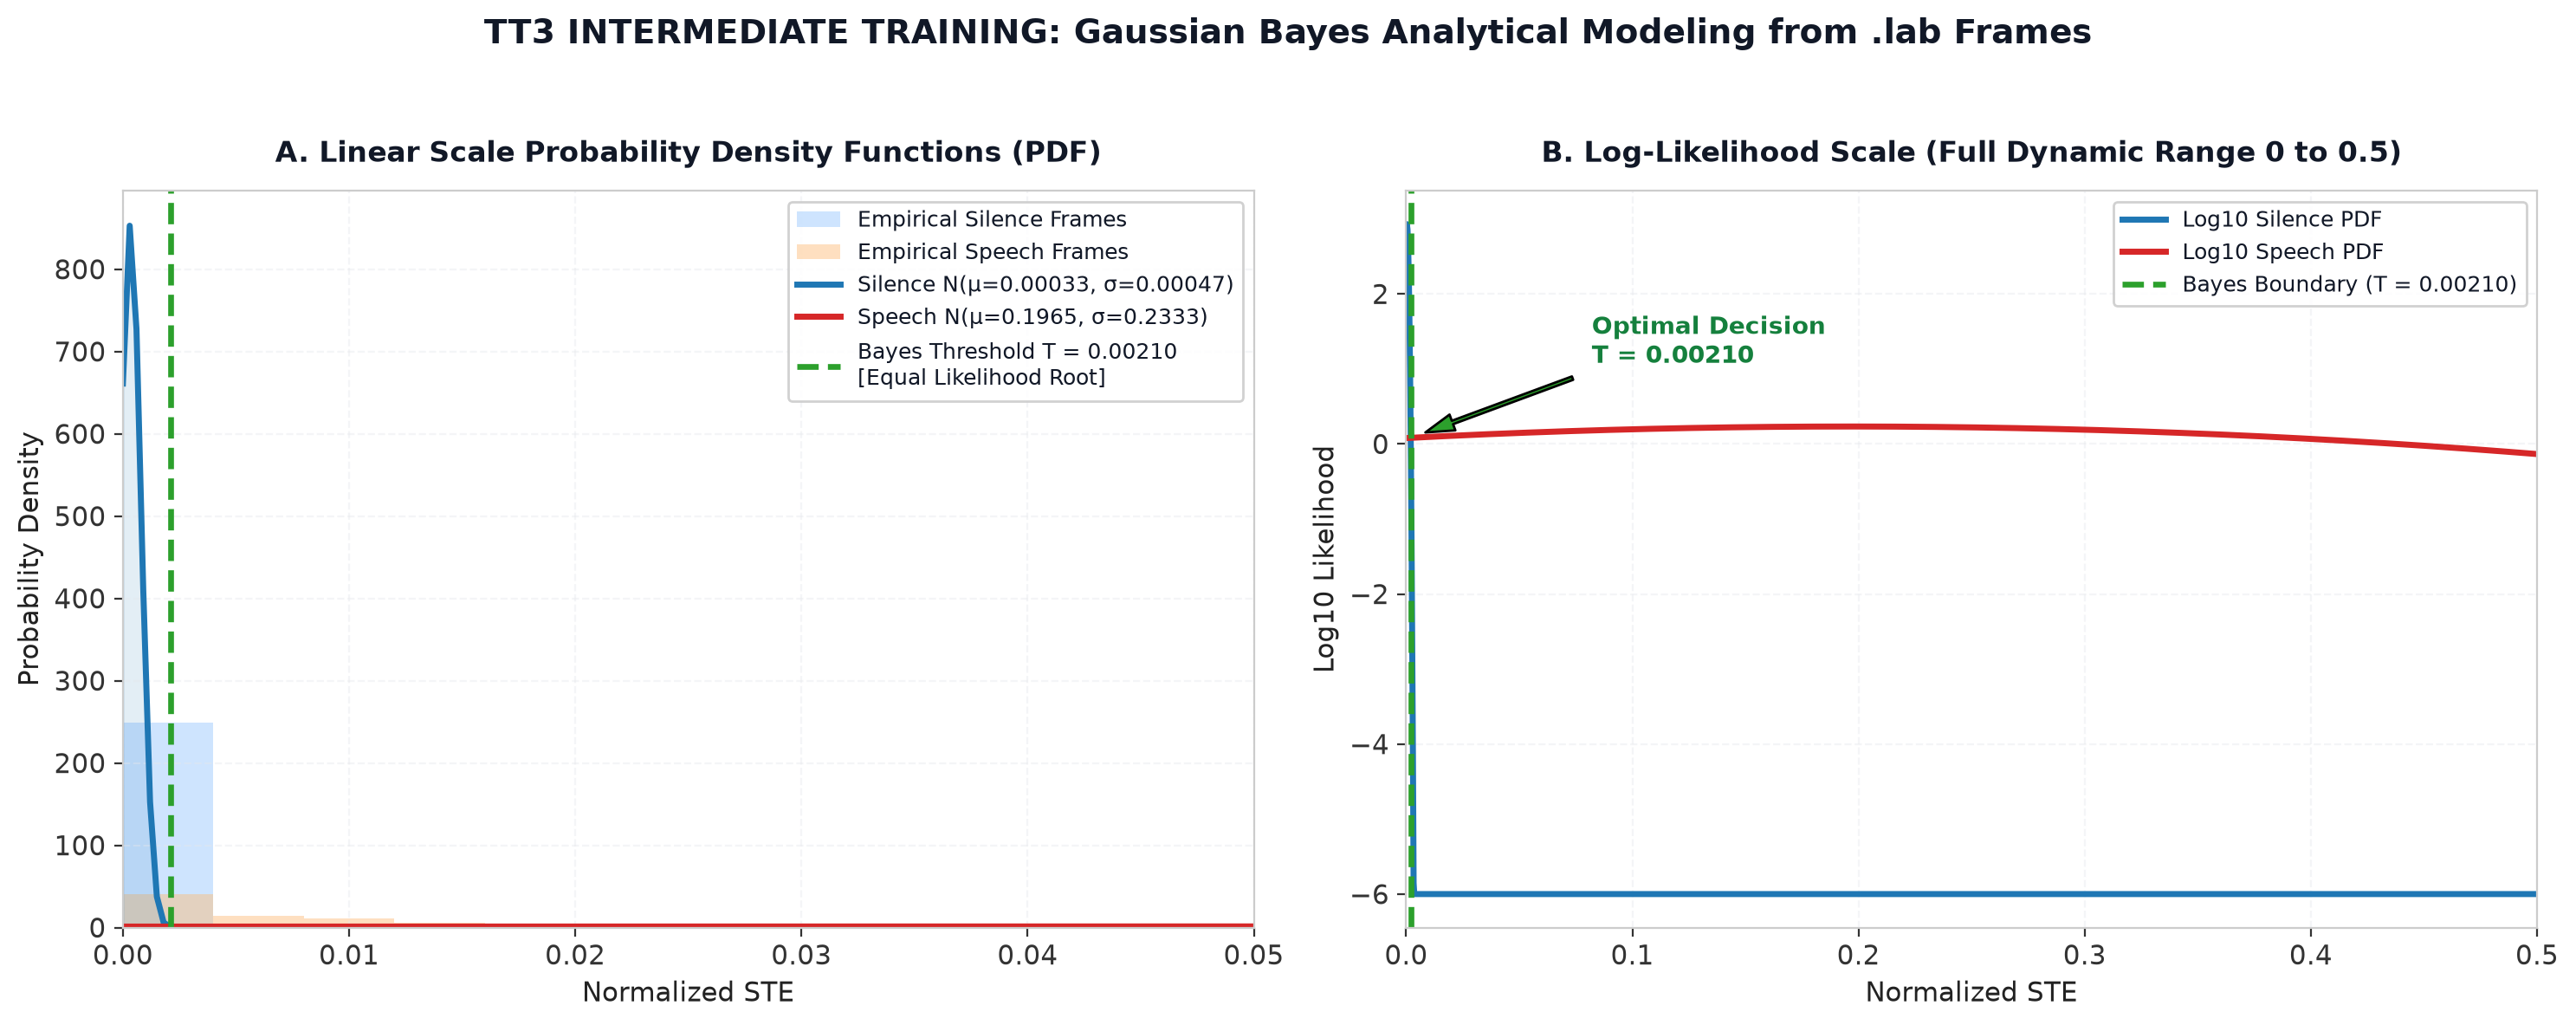
\includegraphics[width=\textwidth, height=4.6cm, keepaspectratio]{figures/tt3_train_gaussian.png}
      \end{tcolorbox}
    \end{column}

    \begin{column}{0.34\textwidth}
      \begin{tcolorbox}[glowcard]
        {\fontsize{8.5pt}{9.5pt}\selectfont\color{cyanGlow}\textbf{Statistical Fit}}\\[2pt]
        {\fontsize{7.5pt}{9pt}\selectfont
        $\bullet$ Fitted Gaussians from 4 train files\\[2pt]
        $\bullet$ Silence $\sigma$ is extremely narrow\\[2pt]
        $\bullet$ Intersection at $p(x|\text{Sil}) = p(x|\text{Sp})$\\[2pt]
        $\bullet$ Closed-form root: $\mathbf{T \approx 0.00202}$}
      \end{tcolorbox}
    \end{column}
  \end{columns}
\end{frame}

% ==============================================================================
% SLIDE 21: APPENDIX 05 - TECHNICAL DEFENSE
% ==============================================================================
\section{APPENDIX 05 $\cdot$ TECHNICAL DEFENSE}
\begin{frame}
  \frametitle{Rebuttal for Critical Examination Questions}
  \begin{columns}[T]
    \begin{column}{0.48\textwidth}
      \begin{tcolorbox}[darkcard]
        {\fontsize{8pt}{9pt}\selectfont\color{cyanGlow}\textbf{Q1: Why not use F0 for boundary cuts?}}\\[2pt]
        {\fontsize{7.5pt}{8.5pt}\selectfont
        Unvoiced consonants (/s/, /t/, /f/) have no pitch F0. Using F0 would truncate initial and trailing phonemes!}
      \end{tcolorbox}
      \vskip3pt
      \begin{tcolorbox}[darkcard]
        {\fontsize{8pt}{9pt}\selectfont\color{cyanGlow}\textbf{Q2: Why did phone\_M2 achieve 0.0 ms MAE?}}\\[2pt]
        {\fontsize{7.5pt}{8.5pt}\selectfont
        Labels [0.53s, 2.52s] coincide with frames 53 \& 252 (10 ms hop grid). It is exact grid snapping, not overfitting!}
      \end{tcolorbox}
    \end{column}

    \begin{column}{0.48\textwidth}
      \begin{tcolorbox}[darkcard]
        {\fontsize{8pt}{9pt}\selectfont\color{cyanGlow}\textbf{Q3: Impact of acoustic noise floor (SNR)?}}\\[2pt]
        {\fontsize{7.5pt}{8.5pt}\selectfont
        Studio (high SNR): Error only 5--10 ms. Phone (low SNR): Trailing breath introduces 20--30 ms boundary lag.}
      \end{tcolorbox}
      \vskip3pt
      \begin{tcolorbox}[darkcard]
        {\fontsize{8pt}{9pt}\selectfont\color{cyanGlow}\textbf{Q4: Why did 1D beat 4D Gaussian in TT3?}}\\[2pt]
        {\fontsize{7.5pt}{8.5pt}\selectfont
        Train set has only 4 files. 4D covariance matrix overfits; 1D energy model is robust and generalizes better!}
      \end{tcolorbox}
    \end{column}
  \end{columns}
\end{frame}

\end{document}
